% Chapter 2 — auto-generated from chapter2_state_of_the_art.md
% Edit the Markdown source, not this file.

\chapter{State of the Art}


\section{The DNS System: Background and Fundamental Concepts}
\label{sec:2.1}

The Domain Name System (DNS) is the distributed directory that translates human-readable domain names into machine-readable information --- primarily IP addresses. As van Rijswijk-Deij et al.~\cite{vanRijswijk2016} observe, "almost all networked services depend on the DNS to store information about the service", from IP address resolution to mail server designation to cryptographic key publication. Understanding its architecture, resolution model, caching behaviour, and resolver ecosystem is a prerequisite for interpreting any DNS measurement study.

\subsection{Hierarchical Structure and Resolution}
\label{subsec:2.1.1}

DNS is organised as a hierarchy whose structure reflects the delegation of administrative authority over portions of the namespace \cite{RFC1034}. The root zone, maintained by ICANN/IANA and operated by twelve root-server organisations, forms the apex of this hierarchy: it contains delegations for every Top-Level Domain (TLD) on the Internet. Below the root, TLDs such as \textit{.com}, \textit{.net}, \textit{.org}, \textit{.fr}, and over 1,500 others each maintain their own authoritative zone. Authoritative name servers at the domain level contain the definitive resource records for specific domains and their subdomains.

Name resolution is carried out by a \textbf{recursive resolver} (also called a full-service resolver), which performs the iterative query sequence on behalf of the client \cite{RFC1034}. When a user or application requests the address of \texttt{www.example.com}, the recursive resolver contacts a root server to obtain the address of the \textit{.com} TLD servers, then the TLD servers to obtain the addresses of the authoritative servers for \texttt{example.com}, and finally the authoritative server to obtain the A or AAAA record for \texttt{www.example.com}. From the client's perspective, this entire process appears as a single request-response exchange.

The recursive resolver may be operated by the client's ISP, by a corporate network gateway, or by a commercial public DNS service such as Google Public DNS (8.8.8.8) or Cloudflare (1.1.1.1). The geographic location of the recursive resolver is a critical parameter for DNS-based CDN routing, as discussed in Section 2.6. Van Rijswijk-Deij et al. (2016) note that the \textit{.com} TLD alone contained approximately 123 million registered names during their measurement period (March 2015 -- January 2016), and that \textit{.com}, \textit{.net}, and \textit{.org} together constitute roughly 50\% of the global DNS name space.

The root zone is protected by DNSSEC since July 2010, establishing the trust anchor for the cryptographic chain that can extend downward to authoritative name servers for individual domains. Twelve of the thirteen logical root server addresses use IP anycast to distribute query load across hundreds of globally distributed physical instances: Jones et al.~\cite{Jones2016} note that the B root is the sole exception, hosted at a single physical location in Los Angeles --- a property exploited in their detection methodology for DNS root manipulation (Section 2.9).

\subsection{Resource Record Types Relevant to Measurement Studies}
\label{subsec:2.1.2}

DNS stores information in typed \textbf{Resource Records} (RR), each serving a distinct purpose \cite{RFC1035}. The record types most relevant to distributed measurement studies are:

\textbf{A and AAAA records} map a domain name to an IPv4 or IPv6 address respectively. A single name may have multiple A or AAAA records, enabling load distribution through round-robin responses and geographic routing through location-aware DNS (different addresses returned depending on the querying resolver's location). This geographic differentiation in A/AAAA responses is one of the primary phenomena this thesis investigates.

\textbf{NS records} designate the authoritative name servers responsible for a DNS zone and are essential for identifying the DNS infrastructure provider responsible for a domain. Van Rijswijk-Deij et al. (2016) include NS records in the OpenINTEL standard query set because changes in NS delegation reveal infrastructure migrations and provider switches.

\textbf{MX records} designate the mail-handling servers for a domain. Van Rijswijk-Deij et al. (2016) use longitudinal MX analysis as one of two case studies for OpenINTEL, tracking the adoption of cloud email services (Google Workspace, Microsoft Exchange Online, Yahoo Mail) across tens of millions of domains over a ten-month period.

\textbf{CNAME records} create an alias pointing from one name to another canonical name. CDNs make extensive use of CNAME chains: a customer domain (\texttt{www.shop.example}) points to a CDN-managed name (\texttt{shop.cdn-provider.net}), allowing the CDN to update routing without requiring the customer to change their DNS configuration.

\textbf{DNSKEY, DS, and RRSIG records} are the DNSSEC record types carrying public keys, delegation signers, and cryptographic signatures respectively. Van Rijswijk-Deij et al. (2016) include all three in the OpenINTEL query set specifically to monitor DNSSEC deployment and key management practices at scale. Their longitudinal data revealed systemic key rollover failures invisible to point-in-time measurements.

\textbf{TXT records} carry free-text information and are used for SPF (Sender Policy Framework), DKIM (DomainKeys Identified Mail), DMARC configuration, and domain validation tokens for certificate authorities. Table~\ref{tab:rr_types} summarises the record types relevant to this thesis's measurement campaign.

\begin{table}[H]
\centering
\small
\begin{tabularx}{\linewidth}{p{1.4cm} p{3.6cm} l X}
\toprule
\textbf{Type} & \textbf{Content} & \textbf{Measured} & \textbf{Relevance for distributed DNS measurement} \\
\midrule
A     & IPv4 address(es)                  & Primary   & Core observable: geographic variation in returned IPs indicates CDN routing or anycast \\
AAAA  & IPv6 address(es)                  & Primary   & Parallel to A; anycast routing may differ between IPv4 and IPv6~\cite{Bortzmeyer2013} \\
NS    & Authoritative name server names   & Weekly    & Identifies DNS provider; enables provider migration tracking and centralisation analysis~\cite{Xu2023} \\
CNAME & Canonical name alias              & Derived   & CDN delegation chain; resolving the chain reveals the CDN operator behind a domain \\
MX    & Mail server hostname(s)           & Quarterly & Cloud email adoption tracking~\cite{vanRijswijk2016}; not geographically differentiated \\
SOA   & Zone authority record             & Quarterly & Zone serial number enables change detection; TTL field reveals operator update policy \\
TXT   & Free-form text                    & Quarterly & SPF/DKIM/DMARC policy; domain ownership verification \\
DNSKEY/DS & DNSSEC public key / delegation & Quarterly & DNSSEC deployment monitoring; broken chains cause SERVFAIL~\cite{vanRijswijk2016} \\
\bottomrule
\end{tabularx}
\caption{DNS Resource Record types relevant to distributed measurement studies, with their measurement frequency in this thesis's campaign. \textit{Primary} types are included in the daily measurement campaign; \textit{weekly} and \textit{quarterly} types are measured in separate batches. References: \cite{RFC1034,RFC1035}.}
\label{tab:rr_types}
\end{table}

\subsection{DNS Caching and TTL: Implications for Active Measurements}
\label{subsec:2.1.3}

Every DNS resource record carries a \textbf{Time To Live} (TTL) value specifying how long a recursive resolver or cache may retain the record before treating it as stale and re-querying the authoritative server \cite{RFC1034,RFC1035}. TTL values reflect a trade-off between server load (longer TTLs mean fewer queries to authoritative servers) and responsiveness (shorter TTLs allow faster propagation of changes). CDNs routinely use short TTLs --- often 60 seconds or less --- to enable rapid traffic redirection, while stable infrastructure records (mail server delegations, authoritative NS records) may carry TTLs of 24 hours or more.

Caching operates at multiple levels: the recursive resolver shared by many clients, the operating system stub resolver, and --- in some implementations --- the application itself. Koch et al.~\cite{Koch2021} emphasise that DNS root records have TTLs measured in days (typically 518,400 seconds = 6 days), meaning that recursive resolvers rarely contact the root in the steady state; most user queries are served from cache.

Two direct implications follow for active DNS measurement studies:

First, if measurements query through a recursive resolver rather than directly at the authoritative server, the response may reflect a cached value from an earlier resolution, not the current authoritative answer. This introduces \textbf{temporal staleness} that must be controlled by querying authoritative servers directly or by accounting for TTL values when interpreting results. Van Rijswijk-Deij et al. (2016) and Bortzmeyer~\cite{Bortzmeyer_tutorial} both explicitly recommend direct authoritative queries when studying DNS record content rather than the user experience.

Second, different probes use different local resolvers with different cache states and different cache populations, meaning the same domain queried "simultaneously" from multiple probes may yield responses that differ due to cache divergence rather than geographic DNS routing intent. Separating these two sources of variation --- intentional geographic routing and incidental caching --- is a methodological challenge that the measurement design of this thesis directly addresses.

\subsection{DNS Resolver Infrastructure and Its Impact on Measurements}
\label{subsec:2.1.4}

The recursive resolver occupies a pivotal position in the DNS resolution chain: it is the infrastructure that CDN authoritative servers query to infer the client's location, and its behaviour determines which cached responses are returned to clients. For distributed DNS measurement studies, understanding the resolver ecosystem is therefore essential.

Xu et al.~\cite{Xu2023} introduce a four-layer taxonomy of client-side DNS infrastructure that reveals the hidden complexity behind what appears to be a simple client-resolver interaction:

\begin{itemize}
  \item \textbf{Forwarding DNS resolvers (FDNS)}: Resolvers deployed close to clients (e.g., ISP edge resolvers) that forward queries to upstream recursive resolvers rather than performing full resolution themselves. They are the entry point for client queries.
  \item \textbf{Recursive DNS resolvers (RDNS)}: Perform full iterative resolution from root to authoritative server. May be collocated with FDNS or geographically distant.
  \item \textbf{Indirect RDNS (iRDNS)}: Higher-level recursive resolvers that serve multiple RDNS instances. Operated by major public DNS providers (Google, Cloudflare) at a small number of locations.
  \item \textbf{Direct RDNS (dRDNS)}: Recursive resolvers that directly contact authoritative servers without going through iRDNS.
\end{itemize}

This layered architecture has a critical implication for measurements: when a RIPE Atlas probe queries through its local resolver (the FDNS), that query may ultimately be resolved by an iRDNS cluster operated by a major provider whose IP address --- not the probe's address --- is presented to the CDN authoritative server. The geographic location of the iRDNS thus determines the CDN's routing decision, not the probe's location. This problem is exacerbated by the extreme concentration documented by Xu et al.~\cite{Xu2023}: over 90\% of forwarding resolvers are backed by fewer than 5\% of indirect recursive resolvers (Section 2.8 expands on this).

In practice, three categories of recursive resolver are commonly encountered by RIPE Atlas probes (Bortzmeyer, n.d., tutorial):

\begin{itemize}
  \item \textbf{ISP resolvers}: Operated by the probe's Internet Service Provider, typically close to the probe geographically. Their IP address is generally a good proxy for the probe's network region, making them preferable for CDN-routing-aware measurements.
  \item \textbf{Public DNS services}: Google Public DNS (8.8.8.8/8.8.4.4), Cloudflare (1.1.1.1/1.0.0.1), Quad9 (9.9.9.9), and others. Their anycast IP addresses resolve to geographically distributed clusters, and the specific cluster that receives a probe's query depends on BGP routing --- which may or may not correlate with the probe's geographic location.
  \item \textbf{Open resolvers}: Resolvers inadvertently left accessible to the public Internet. Bortzmeyer~\cite{Bortzmeyer_tutorial} advises against using open resolvers for structured measurement, both for ethical reasons (they are open by negligence, not intent) and for reliability reasons (their behaviour is unpredictable).
\end{itemize}

For this thesis, these distinctions motivate the design choice to query authoritative name servers directly --- bypassing the resolver layer entirely --- in order to control for resolver-location effects and measure the geographic DNS responses that would be returned to clients regardless of their resolver infrastructure.
\bigskip
\section{DNS Measurements: Active and Passive Paradigms}
\label{sec:2.2}

The literature broadly distinguishes two fundamental measurement paradigms: \textbf{passive} measurements, which analyse DNS traffic as it flows through existing infrastructure without injecting artificial queries, and \textbf{active} measurements, which deliberately generate queries from controlled vantage points to study the DNS system directly. Each paradigm offers complementary trade-offs in terms of coverage, geographic control, reproducibility, and ethical impact.

\subsection{Passive DNS Measurement}
\label{subsec:2.2.1}

Passive DNS (pDNS) systems capture DNS queries and responses at existing resolvers or network transit points --- Internet Exchange Points, ISP recursive resolvers, or authoritative name servers --- without generating artificial traffic. Van der Toorn et al. (2018) describe passive DNS as providing a "live" view of actual DNS usage: observations reflect queries generated by real users, making passive DNS well suited for studying organic DNS behaviour, detecting anomalies in query patterns, and identifying malicious domains that are actively used. Commercial passive DNS services such as Farsight Security's DNSDB aggregate billions of DNS responses daily from voluntarily participating resolvers worldwide; these datasets are widely used in security research for botnet tracking, phishing detection, and malware infrastructure analysis.

The advantages of passive DNS measurement are its non-intrusiveness (no artificial traffic is injected, eliminating any concern about overloading queried servers) and its ability to capture real traffic volumes and timing. These properties make it the preferred approach for traffic analysis and security forensics.

However, passive DNS carries fundamental limitations for the geographic DNS response variation research question at the centre of this thesis:

\textbf{Access constraints}: Passive observation requires privileged access to DNS traffic transit points --- ISP resolvers, IXPs, or authoritative servers --- which is typically available only to operators of that infrastructure or through specific research partnerships. Independent academic researchers face significant logistical barriers to deploying passive observation at geographically diverse points.

\textbf{Geographic blindness}: A passive sensor observes only the traffic that passes through its observation point. Van Rijswijk-Deij et al. (2016) explicitly identify this as the core limitation of passive approaches: single-vantage-point passive DNS cannot reveal how DNS responses differ across geographic locations, which is precisely the question distributed active measurement is designed to answer.

\textbf{Domain selection bias}: Passive DNS observes only domains that are actually queried by the local user population. A controlled comparative study of a predefined domain set --- such as measuring all 10,000 Tranco top domains --- is impossible with passive measurement, since many domains in any fixed set will receive no organic traffic from any given observation point.

\textbf{Privacy constraints}: DNS traffic contains implicit information about user browsing behaviour. Collection and retention of DNS traffic raises significant privacy concerns under data protection regulations such as the GDPR, constraining the scope of permissible passive DNS research and the granularity at which data can be stored.

\subsection{Active DNS Measurement}
\label{subsec:2.2.2}

Active measurement deliberately sends DNS queries to predefined domain targets from controlled vantage points. Van Rijswijk-Deij et al. (2016) motivate this paradigm by observing that "studying the state of large parts of the DNS over time reveals valuable information about the evolution of the Internet", a goal that only active measurement can achieve comprehensively and reproducibly.

The core advantages of the active approach are:

\textbf{Full domain coverage}: Any domain in a TLD zone file, or any domain on a research list such as Tranco, can be measured regardless of whether it has organic traffic. This enables systematic, bias-free coverage of predefined domain sets (van Rijswijk-Deij et al., 2016, Goal G1).

\textbf{Reproducibility}: The same set of domains, record types, vantage points, and measurement frequency can be reproduced identically across multiple time periods and by different research groups. This is a fundamental criterion of scientific research that passive measurements --- tied to organic traffic patterns --- cannot guarantee.

\textbf{Geographic control}: Vantage points can be explicitly selected to cover specific geographic regions or network positions of interest, enabling the comparison of DNS responses across locations. This is the central capability leveraged by this thesis.

\textbf{Parameter control}: The experimenter fully controls technical measurement parameters: DNS query type (A, AAAA, NS, MX, SOA), use of DNSSEC validation, inclusion of EDNS options (NSID, ECS), whether to query through a local resolver or directly at an authoritative server, and measurement frequency.

\textbf{Infrastructure impact quantification}: Van Rijswijk-Deij et al. (2016) empirically quantify the impact of OpenINTEL's active measurements on the global DNS infrastructure. Despite generating at least 1.85 billion queries per day for the \textit{.com} TLD alone (123 million names $\times$ 14 query types per name, plus recursion overhead), the traffic generated represents only \textbf{0.3\% to 1.6\%} of total DNS traffic observed on the authoritative servers analysed. No correlation between OpenINTEL measurement peaks and server performance degradation is detectable. This result establishes that well-designed active measurements --- appropriately paced and sized --- have a negligible impact on the infrastructure being studied.

The scientific value of active measurements is further illustrated by van der Toorn et al.~\cite{vanderToorn2018}, who apply OpenINTEL data (measuring more than 60\% of the global DNS namespace daily) to detect snowshoe spam domains using supervised machine learning. Snowshoe spam distributes sending across many domains, each with low individual traffic --- precisely the pattern that makes these domains invisible to passive DNS (which only observes domains with organic query traffic). The active measurement approach reveals the structural DNS patterns (many A records per domain, SPF configurations with many hosts) that characterise snowshoe spam infrastructure even before any spam has been sent. The result is a detection precision of over \textbf{93\%} with a \textbf{100-day lead} over existing blacklists --- a capability exclusive to the active measurement paradigm.

\subsection{Ethical Dimensions of Active Measurement}
\label{subsec:2.2.3}

Active measurements using volunteer-hosted infrastructure raise ethical responsibilities that must be explicitly addressed in the research design. Kisteleki et al.~\cite{Kisteleki2016} provide the primary ethical framework for RIPE Atlas measurements, grounding it in the \textbf{Menlo Report} (2012) --- which extends the Belmont Report (1978) principles of beneficence, justice, and respect for persons to ICT research --- and in the work of Allman and Partridge (2016), who propose formal ethics review sections in measurement papers.

The core principle articulated by Kisteleki et al.~\cite{Kisteleki2016} is that RIPE Atlas probe hosts are volunteers whose internet connections are used to generate measurement traffic. Researchers bear responsibility for the traffic those connections produce, not only in terms of volume but in terms of the legal and social risk that traffic creates for the probe host in their jurisdiction. This is illustrated by the "Ebonia" case: a researcher planned to use probes in a politically volatile region to measure access to socially sensitive websites, until colleagues highlighted that the probe hosts --- not the researcher --- would bear the legal risk of that traffic. The study was redesigned with less sensitive query targets. Kisteleki et al.~\cite{Kisteleki2016} further describe a case where RIPE NCC required that a Google search measurement study use only "risk-free search terms such as 'cat' and 'dog'" rather than the politically sensitive terms initially proposed.

RIPE NCC enforces these principles institutionally: HTTP measurements are restricted to RIPE Atlas anchors (trusted, known-good destinations) by default, and access to the platform can be terminated for research that generates complaints about unethical behaviour \cite{Kisteleki2016}.

For this thesis, these principles translate to concrete methodological design choices: the domain corpus is drawn from the Tranco list of popular, publicly accessible domains; no politically sensitive, jurisdictionally censored, or legally ambiguous content is queried; measurement frequency is set to respect DNS TTLs; and all measurement traffic is identifiable as RIPE Atlas-sourced, allowing authoritative server operators to filter if needed.

\subsection{Specific Technical Challenges of Distributed Active DNS Measurements}
\label{subsec:2.2.4}

Beyond the general advantages and limitations, distributed active DNS measurements from geographically dispersed probes introduce specific technical challenges that must be addressed in the measurement design.

\textbf{Measurement desynchronisation}: Holterbach et al.~\cite{Holterbach2015} demonstrate that when a "simultaneous" measurement is launched from multiple RIPE Atlas probes, the actual DNS queries are not sent at the same instant. Under heavy concurrent platform load, the spread between the first and last probe completing a one-off measurement can reach \textbf{up to one hour}. This matters when studying dynamic DNS properties (CDN traffic shifts, DNS record changes) that evolve on timescales comparable to the measurement spread. Mitigation strategies include using scheduled periodic measurements (rather than one-off) and repeating measurements to identify transient anomalies.

\textbf{Heterogeneous resolver behaviour}: Each RIPE Atlas probe uses the resolver configured by its host --- typically the probe's ISP resolver. These resolvers have heterogeneous characteristics: different TTL caching policies, different DNSSEC validation support, different EDNS compliance, and potentially different filtering policies. Bajpai et al.~\cite{Bajpai2017} expose this through the RIPE Atlas tag system: tags such as \texttt{system-resolves-a-correctly} and \texttt{system-resolver-mangles-case} identify probes whose resolvers exhibit abnormal behaviour. Measurements that rely on consistent resolver behaviour across all probes must filter by these system tags. Alternatively, specifying an explicit resolver (e.g., a known public resolver) in the measurement definition bypasses local resolver variability.

\textbf{Cache state divergence}: Because each probe's resolver independently caches DNS responses, the cache state of two probes measuring the same domain at the same time may differ substantially --- one resolver may have cached an older version of a record while another has a fresh response. This source of variation can mimic geographic routing differences. Querying authoritative servers directly, rather than through local resolvers, eliminates this ambiguity by bypassing resolver caches entirely.

\textbf{IPv4/IPv6 measurement parallelism}: Anycast routing tables for IPv4 and IPv6 are maintained independently, and the same anycast service may direct IPv4 and IPv6 queries to different physical instances (Section 2.5.3). Bortzmeyer~\cite{Bortzmeyer2013} documents this empirically for d.nic.fr: the dominant anycast instance reverses between the two protocols. Measurement campaigns that combine IPv4 and IPv6 probes without distinguishing between them will obtain a conflated view of anycast instance distribution. Dual-stack measurements should be conducted and analysed separately.
\bigskip
\section{OpenINTEL: Large-Scale Forward DNS Measurement}
\label{sec:2.3}

OpenINTEL, developed at the University of Twente in collaboration with SURFnet, SIDN (the \textit{.nl} registry), and (since 2018) NLnet Labs, is the most comprehensive active DNS measurement infrastructure for longitudinal studies of the global DNS \cite{vanRijswijk2016,vanRijswijk2018blog}. Its architecture and operational experience directly inform the design of this thesis's measurement system.

\subsection{Design Goals, Challenges, and Architecture}
\label{subsec:2.3.1}

Van Rijswijk-Deij et al. (2016) define seven research goals (G1--G7) and five technical challenges (C1--C5) that shaped OpenINTEL's design. The core goals are: measuring \textbf{every domain in a TLD} once per day (G1, G4), covering even the largest TLD --- \textit{.com} with 123 million names (G2) --- querying a \textbf{fixed set of relevant resource records} per domain (G3), storing at least one year of data for longitudinal analysis (G5), and supporting efficient analysis at scale using modern data processing tools (G6, G7).

The fixed query set (Table I of van Rijswijk-Deij et al., 2016) includes A, AAAA, NS, MX, SOA, DNSKEY, DS, and RRSIG record types. This selection was chosen to cover the most common DNS uses with the minimum number of queries: IPv4 and IPv6 addressing, mail routing, zone delegation, and DNSSEC cryptographic infrastructure. Each domain thus requires 14 queries (8 record types, some requiring multiple query forms), producing the primary challenge: querying 123 million \textit{.com} names $\times$ 14 queries = \textbf{at least 1.85 billion DNS queries per day} for \textit{.com} alone.

Three architectural choices address this challenge:

\textbf{DNS software selection}: Rather than a bare-metal approach that would require re-implementing DNS recursion (risking bugs that compromise measurement correctness), OpenINTEL uses off-the-shelf DNS software: LDNS as a stub resolver for sending individual queries, and Unbound as a full recursive resolver. This prioritises correctness and robustness (Challenge C4) over maximum throughput.

\textbf{Distributed worker architecture}: A central orchestration component coordinates a swarm of worker nodes implemented as virtual machines, enabling horizontal scaling. The distributed design allows the system to handle both the current query volume and future TLD growth (Goal G7 and Challenge C5), and in principle permits geographic distribution of workers for measurements requiring local vantage points.

\textbf{Query pacing}: To avoid overloading authoritative DNS servers for individual TLDs --- particularly the root servers and TLD servers that receive a query for every measured domain --- queries are distributed over time rather than batched. This pacing is essential for meeting Challenge C2: the traffic OpenINTEL generates must not be an "unacceptable burden" on the global DNS infrastructure.

\textbf{Data storage}: Results are serialised in \textbf{Apache Avro} format (self-describing, compressed) and subsequently converted to \textbf{Apache Parquet} for efficient columnar analysis within the Hadoop ecosystem (Goal G6). The estimated storage volume for \textit{.com} alone is 123M $\times$ 14 queries $\times$ \textasciitilde{}150 bytes/query $\approx$ 240 GB/day. For multi-year longitudinal studies, this necessitates petabyte-scale storage, addressed by the Hadoop cluster added in September 2015 \cite{vanRijswijk2018blog}.

\subsection{Scale, Operational Reach, and Published Results}
\label{subsec:2.3.2}

The first complete OpenINTEL measurement day was \textbf{21 February 2015}, with regular daily measurements beginning 1 March 2015 \cite{vanRijswijk2018blog}. Coverage expanded progressively: initial deployment covered \textit{.com}, \textit{.net}, and \textit{.org} (50\% of the global DNS namespace); subsequent phases added major country-code TLDs and additional gTLDs; by 2018, all generic TLDs were included. As of this thesis's writing, the platform has accumulated over ten years of continuous daily DNS measurements, constituting a unique longitudinal dataset for Internet infrastructure research.

Three award-winning publications illustrate the platform's research value:

\begin{itemize}
  \item \textbf{DDoS protection adoption} (Jonker et al., IMC 2016): Using 1.5 years of OpenINTEL data, Jonker et al. study how domains adopt DDoS mitigation services over time, revealing concentration patterns in DDoS protection infrastructure \cite{vanRijswijk2018blog}.
\end{itemize}

\begin{itemize}
  \item \textbf{DNSSEC key management failures} (van Rijswijk-Deij et al., USENIX Security 2017, Distinguished Paper Award): A 21-month longitudinal analysis reveals that many DNSSEC-signed domains suffer from key rollover failures --- domains whose signing keys expire but are not replaced, leaving them cryptographically unsigned despite appearing in signed zones. These findings, which demonstrate systemic operational failures in DNSSEC implementation, are only possible through continuous active measurement: a point-in-time study would capture each domain's state at a single moment without revealing the temporal dynamics of key management \cite{vanRijswijk2018blog}.
\end{itemize}

\begin{itemize}
  \item \textbf{Snowshoe spam detection} (van der Toorn et al., NOMS 2018, Best Paper Award): 180 days of OpenINTEL data, combined with supervised machine learning, detect snowshoe spam domains with 93\%+ precision and a 100-day lead over traditional blacklists. The approach is validated through three-month production deployment in a major Dutch network operator's mail filter \cite{vanderToorn2018}.
\end{itemize}

The \textbf{Research Data Netherlands Prize}, received in November 2018, further validates OpenINTEL's position as a premier research infrastructure \cite{vanRijswijk2018blog}.

\textbf{OpenINTEL case study --- cloud email adoption}: Van Rijswijk-Deij et al. (2016) use OpenINTEL's longitudinal MX record data as a concrete demonstration of the platform's capacity to track large-scale changes in Internet infrastructure. Over a ten-month period (March 2015 to January 2016), they observe the MX records of tens of millions of domains in the \textit{.com}, \textit{.net}, and \textit{.org} TLDs, identifying which mail server infrastructure each domain delegates its inbound email to. Three cloud email services --- Google Workspace (G Suite at the time), Microsoft Exchange Online, and Yahoo Mail --- are each identifiable by the distinctive MX hostname patterns they assign to their customers (e.g., \texttt{aspmx.l.google.com} for Google Workspace, \texttt{*.protection.outlook.com} for Microsoft). The longitudinal daily time series reveals the adoption trajectory of each service: which TLD registrant communities adopt each service first, how adoption velocity differs across TLDs, and whether adoption events are correlated with external announcements (product launches, pricing changes). This application demonstrates a category of research entirely unavailable to point-in-time measurement or passive DNS: the ability to observe and quantify the timing and pace of large-scale infrastructure migration decisions by millions of domain operators worldwide. For this thesis, the same principle applies to DNS resolver infrastructure: longitudinal active measurement can reveal when CDN operators reconfigure their DNS-based routing policies, when new anycast PoPs are deployed, and when domain operators migrate between DNS providers --- events that are instantaneous from a point-in-time perspective but become legible through continuous active measurement.

\textbf{Critical limitation --- geographic monoculture}: All OpenINTEL measurements are performed from \textbf{a single vantage point in the Netherlands}. This architecture provides exhaustive, unbiased TLD-wide domain coverage but makes \textbf{geographic variation in DNS responses completely invisible}. A CDN authoritative server responding to OpenINTEL queries always sees the same source IP address: the Dutch measurement server's address. Whether that domain returns different IP addresses to probes in Japan, Brazil, or South Africa --- the core question of this thesis --- cannot be answered from OpenINTEL data alone. Van Rijswijk-Deij (2018) explicitly identifies the single-vantage-point design as a limitation of the platform. This gap, the absence of spatial diversity in existing longitudinal DNS measurement infrastructure, is the primary motivation for the geographically distributed RIPE Atlas approach developed in this thesis.
\bigskip
\section{Distributed Measurement Platform: RIPE Atlas}
\label{sec:2.4}

RIPE Atlas is an Internet measurement platform operated by RIPE NCC, consisting of a globally distributed network of hardware probes hosted by volunteers in home networks, ISPs, IXPs, and academic institutions. It provides the spatial diversity that OpenINTEL lacks and serves as the primary measurement infrastructure for this thesis.

\subsection{Platform Overview, Hardware, and Comparison with Alternatives}
\label{subsec:2.4.1}

\textbf{Scale and hardware}: As of the analysis by Nosyk et al.~\cite{Nosyk2024}, RIPE Atlas comprises \textbf{12,892 active probes} distributed across \textbf{178 countries}, generating approximately \textbf{1.3 billion measurement results per day}. The platform has grown substantially since its launch: Holterbach et al.~\cite{Holterbach2015} report 6,700 public probes in 197 countries as of April 2015, and Bajpai et al.~\cite{Bajpai2017} report 9,100 probes as of January 2017. Three hardware generations of probes have been deployed \cite{Holterbach2015}: Versions 1 and 2 are Lantronix XPort Pro devices with 167 MHz CPU and 8--16 MB RAM; Version 3 is a TP-Link TL-MR3020 router with a 400 MHz CPU, 32 MB RAM, and 4 MB NAND flash, making it substantially more powerful. By 2015, v3 probes hosted approximately two-thirds of all measurements, though v1 and v2 probes remained non-negligible \cite{Holterbach2015}.

\textbf{Credit system}: Platform access is governed by a credit economy. Probe hosts earn credits for each hour their probe is connected and available for measurements; these credits can be spent to create user-defined measurement campaigns. Holterbach et al.~\cite{Holterbach2015} describe the cost model: traceroutes are the most expensive measurement type; scheduled repeated measurements cost approximately half as much as equivalent one-off measurements. Built-in measurement types available to all users include ping, traceroute, DNS, and SSL certificate retrieval.

\textbf{Comparison with alternative measurement platforms}: Bajpai et al.~\cite{Bajpai2017} survey the landscape of Internet measurement platforms active as of January 2017. \textbf{CAIDA Archipelago (Ark)} consists of approximately 170 hardware monitors coordinated for Internet topology mapping; it is smaller and more specialised than RIPE Atlas. \textbf{SamKnows} deploys approximately 70,000 hardware probes in collaboration with ISPs and regulators to assess broadband performance; probes are ISP-deployed rather than volunteer-hosted, limiting independence from the monitored infrastructure. \textbf{DIMES} and \textbf{iPlane} are software-based platforms focused on topology mapping. \textbf{BISmark} from Georgia Tech deploys approximately 420 probes for home network characterisation. For anycast census studies, Cicalese et al.~\cite{Cicalese2015} use approximately 300 active PlanetLab vantage points --- fewer than RIPE Atlas but with greater flexibility for scanning-style experiments. Bajpai et al.~\cite{Bajpai2017} conclude that RIPE Atlas is "the largest open platform today" and plays "a critical role in not only providing operational support to network operators but also facilitating measurement-based research". For DNS-focused studies specifically, RIPE Atlas's built-in DNS measurement type and the geographic diversity of its probe population make it the preferred platform. Table~\ref{tab:platforms} summarises the key characteristics of the main alternatives.

\begin{table}[H]
\centering
\small
\begin{tabularx}{\linewidth}{p{2.6cm} r p{2.0cm} p{1.8cm} X}
\toprule
\textbf{Platform} & \textbf{Probes} & \textbf{Countries} & \textbf{DNS native} & \textbf{Notes} \\
\midrule
RIPE Atlas       & $\approx$12,900 & 178 & Yes & Volunteer hardware probes; credit economy; open academic access~\cite{Nosyk2024} \\
CAIDA Ark        & $\approx$170    & 60+ & No  & Topology-focused; not volunteer-based; limited DNS support~\cite{Bajpai2017} \\
SamKnows         & $\approx$70,000 & 50+ & No  & ISP-deployed; broadband QoS focus; not openly accessible~\cite{Bajpai2017} \\
PlanetLab        & $\approx$300    & 60+ & No  & Software VMs; flexible but low reliability; largely inactive~\cite{Cicalese2015} \\
BISmark          & $\approx$420    & 40+ & No  & Home-network focus (Georgia Tech); limited geographic diversity~\cite{Bajpai2017} \\
\bottomrule
\end{tabularx}
\caption{Comparison of distributed Internet measurement platforms relevant to DNS studies. Probe counts as of 2024 for RIPE Atlas~\cite{Nosyk2024} and approximately 2017 for others~\cite{Bajpai2017}. RIPE Atlas is the only platform with native DNS measurement support and open academic access at global scale.}
\label{tab:platforms}
\end{table}

\subsection{Probe Selection and the Tag System}
\label{subsec:2.4.2}

Selecting appropriate vantage points is a critical methodological decision that directly affects the validity and interpretability of measurement results. Bajpai et al.~\cite{Bajpai2017} analyse the tag-based filtering system introduced by RIPE Atlas in July 2014 (available for probe selection since October 2014) and identify important differences in tag reliability.

\textbf{System tags} are automatically assigned by the RIPE Atlas infrastructure based on the results of continuous built-in measurements. Table I of Bajpai et al.~\cite{Bajpai2017} lists the default measurements run by every probe, including ping and traceroute to root servers and Atlas infrastructure, DNS queries to all root servers, and SSL certificate retrieval. From these measurements, RIPE Atlas derives and updates system tags every four hours. Examples include \texttt{system-ipv4-works} (IPv4 connectivity verified), \texttt{system-ipv6-works} (IPv6 connectivity verified), \texttt{system-resolves-a-correctly} (probe's local resolver returns correct A records), and \texttt{system-resolver-mangles-case} (resolver modifies the case of query names, indicating potential anomalous behaviour). Because system tags are derived from actual measurements and refreshed frequently, they reliably reflect the current network state of the probe.

\textbf{User tags} are applied voluntarily by probe hosts to describe their deployment context. Bajpai et al.~\cite{Bajpai2017} find that only \textbf{\textasciitilde{}2.8\% of probe hosts ever update their user tags} after initially setting them. User tags therefore frequently become stale --- a probe initially tagged as "home DSL" may now be on a fibre connection, but the tag remains unchanged. Researchers relying on user tags for probe selection risk drawing on outdated classification information. The practical recommendation from Bajpai et al.~\cite{Bajpai2017} is to prioritise system tags over user tags whenever system tag equivalents exist.

Using the \texttt{system-ipv6-works} tag to select dual-stacked probes, Bajpai et al.~\cite{Bajpai2017} identify approximately \textbf{2,300 probes} with working IPv6 connectivity as of January 2017, spanning \textbf{88 countries} and \textbf{822 Autonomous Systems}. Of these, 83\% are connected within access networks (DSL, cable, or fibre), and 91\% are concentrated in the RIPE (Europe/Middle East) and ARIN (North America) regions. Countries such as Belgium and Japan are explicitly identified as underrepresented for IPv6 measurement studies relative to their actual IPv6 user populations.

Bajpai et al.~\cite{Bajpai2017} propose a practical probe selection protocol applicable to any RIPE Atlas study requiring geographic diversity and connectivity reliability. The recommended sequence is: (1) apply the relevant connectivity system tags (\texttt{system-ipv4-works}, \texttt{system-ipv6-works}, \texttt{system-resolves-a-correctly}) to exclude probes with known connectivity or resolver problems; (2) apply any study-specific system tags (e.g., \texttt{system-ipv4-stable-1d} for probes with stable 24-hour IPv4 connectivity); (3) stratify the remaining probe pool geographically to achieve the desired regional balance, accounting for the known 91\% Europe/North America concentration; (4) draw a random sample from each geographic stratum. This stratified-sampling protocol avoids the alternative of accepting RIPE Atlas's natural distribution, which would produce a dataset dominated by European and North American probes and yield unreliable results for Africa, Latin America, and Southeast Asia. For studies of geographic DNS variation specifically, the geographic stratification step is the most critical: ensuring that each inhabited continent has a minimum number of probes guarantees that regional DNS responses --- which may be qualitatively different from European responses --- are captured with statistical confidence. Bajpai et al.~\cite{Bajpai2017} further note that selecting probes by country (rather than by geographic region) provides finer granularity but risks selecting all probes from a single ASN in small countries, reducing network diversity; the recommended trade-off is geographic stratification at the continent level with AS diversity as a secondary constraint.

\subsection{DNS Measurement Capabilities and Notable Applications}
\label{subsec:2.4.3}

DNS is one of RIPE Atlas's primary built-in measurement types. Every probe continuously runs default DNS measurements to all thirteen DNS root server addresses, querying for SOA, \texttt{version.bind}, \texttt{hostname.bind}, and \texttt{id.server} in both standard (IN) and CHAOS classes, as well as over TCP \cite{Bajpai2017}. User-defined DNS measurements extend this to any domain, any record type, any target resolver (the probe's local resolver or a specified IP address), and optionally include EDNS options such as NSID or DNSSEC OK flags.

Nosyk et al.~\cite{Nosyk2024} quantify the DNS measurement activity of RIPE Atlas as of 2024: approximately \textbf{88,000 user-defined DNS measurement instances are executed daily}, in addition to the continuous built-in measurements. The platform generates approximately \textbf{1.3 billion results per day} across all measurement types.

Nosyk et al.~\cite{Nosyk2024} further characterise the composition of RIPE Atlas DNS measurements. They distinguish between measurements targeting \textbf{public resolvers} (querying 8.8.8.8, 1.1.1.1, or similar services), measurements querying \textbf{local resolvers} (the probe's own ISP resolver), and measurements querying \textbf{authoritative servers} directly. Each category provides a different perspective on DNS infrastructure: public resolver measurements capture the performance and correctness of centralised resolver infrastructure; local resolver measurements reflect the DNS experience of typical end users in that network; and authoritative server measurements reveal the DNS responses returned at the authoritative layer, independent of resolver mediation. Nosyk et al.~\cite{Nosyk2024} observe that the distribution of measurement types varies substantially by user: some researchers deploy systematic targeted campaigns while others run exploratory single-run measurements. The operational analysis also characterises measurement temporal patterns: most user-defined measurements run during peak working hours in Europe and North America, creating temporal concentration that interacts with the interference effects documented by Holterbach et al.~\cite{Holterbach2015}. Nosyk et al.~\cite{Nosyk2024} further derive practical guidelines for measurement design: selecting probes using system tags (not user tags), scheduling campaigns at off-peak times to reduce interference, validating probe geolocation against external databases, and cross-referencing DNS non-responses against connectivity indicators to distinguish censorship from measurement failure.

Several published applications illustrate the analytical reach of RIPE Atlas for DNS research:

\textbf{DNS root manipulation detection} \cite{Jones2016}: Using approximately 8,000 Atlas probes in 2,755 Autonomous Systems across 189 countries, Jones et al. detect in-path DNS proxies by comparing ICMP ping RTT to the B root server (the only non-anycasted root, physically located in Los Angeles) with the DNS query RTT observed by the same probe. A Kenyan ISP's transparent proxy is identified by the anomaly: DNS query RTT is 14 ms while the ping RTT to the actual B root in Los Angeles is 318 ms --- a factor of 23, which is physically impossible unless the DNS response originates from a local proxy. Eleven probes in total return unexpected \texttt{HOSTNAME.BIND} identities, indicating ISP-level DNS interception or local root mirrors. The study further identifies that 1.7\% of Atlas probes have inconsistent geolocation data, highlighting the importance of probe metadata validation.

\textbf{Internal domain names and name collision risk} \cite{Boswell2024}: This study leverages the concentration of RIPE Atlas probes in home networks --- typically treated as a bias to be corrected --- as a deliberate research feature. The authors design a four-step active measurement methodology combining traceroute-based gateway discovery, CHAOS TXT queries for \texttt{hostname.bind} to fingerprint gateway models, and reverse DNS queries to detect internal names resolved by home routers. Applied to all IPv4 RIPE Atlas probes in early 2024, the study discovers 3,092 distinct internal domain names used by 4,305 probes (50.86\% of probes tested). The top ten internal names are all related to AVM FRITZ!Box routers (e.g., \texttt{fritz.box}, \texttt{myfritz.box}), reflecting the gateway's dominance in the European market. Of the internal names discovered, 34.51\% use a TLD not currently delegated in the public DNS --- a significant name collision risk if those TLDs are later delegated, as demonstrated by the concrete \texttt{.box} TLD delegation in August 2023.

\textbf{Anycast instance characterisation} (Bortzmeyer, 2013; Finnegan, 2018; Edgecast, 2017): described in Section 2.5.

\subsection{Geographic Bias and Measurement Interference}
\label{subsec:2.4.4}

Two systematic platform-level limitations must be accounted for in any RIPE Atlas measurement methodology.

\textbf{Geographic concentration}: Nosyk et al.~\cite{Nosyk2024} quantify the geographic distribution of RIPE Atlas probes: \textbf{Germany and the USA together account for 28\%} of all active probes, and Europe and North America together account for the majority of the platform. The Bajpai et al.~\cite{Bajpai2017} analysis confirms that 91\% of dual-stacked probes are concentrated in the RIPE (Europe/Middle East) and ARIN (North America) regions. Africa, Latin America, and Central/Southeast Asia are substantially underrepresented relative to their shares of the global Internet user population. This geographic concentration means that any global inference from RIPE Atlas data must account for regional sampling bias: results will be statistically robust for Europe and North America but less reliable for underrepresented regions. Figure~\ref{fig:ripe_atlas_distribution} maps this distribution.

\begin{figure}[tp]
  \centering
  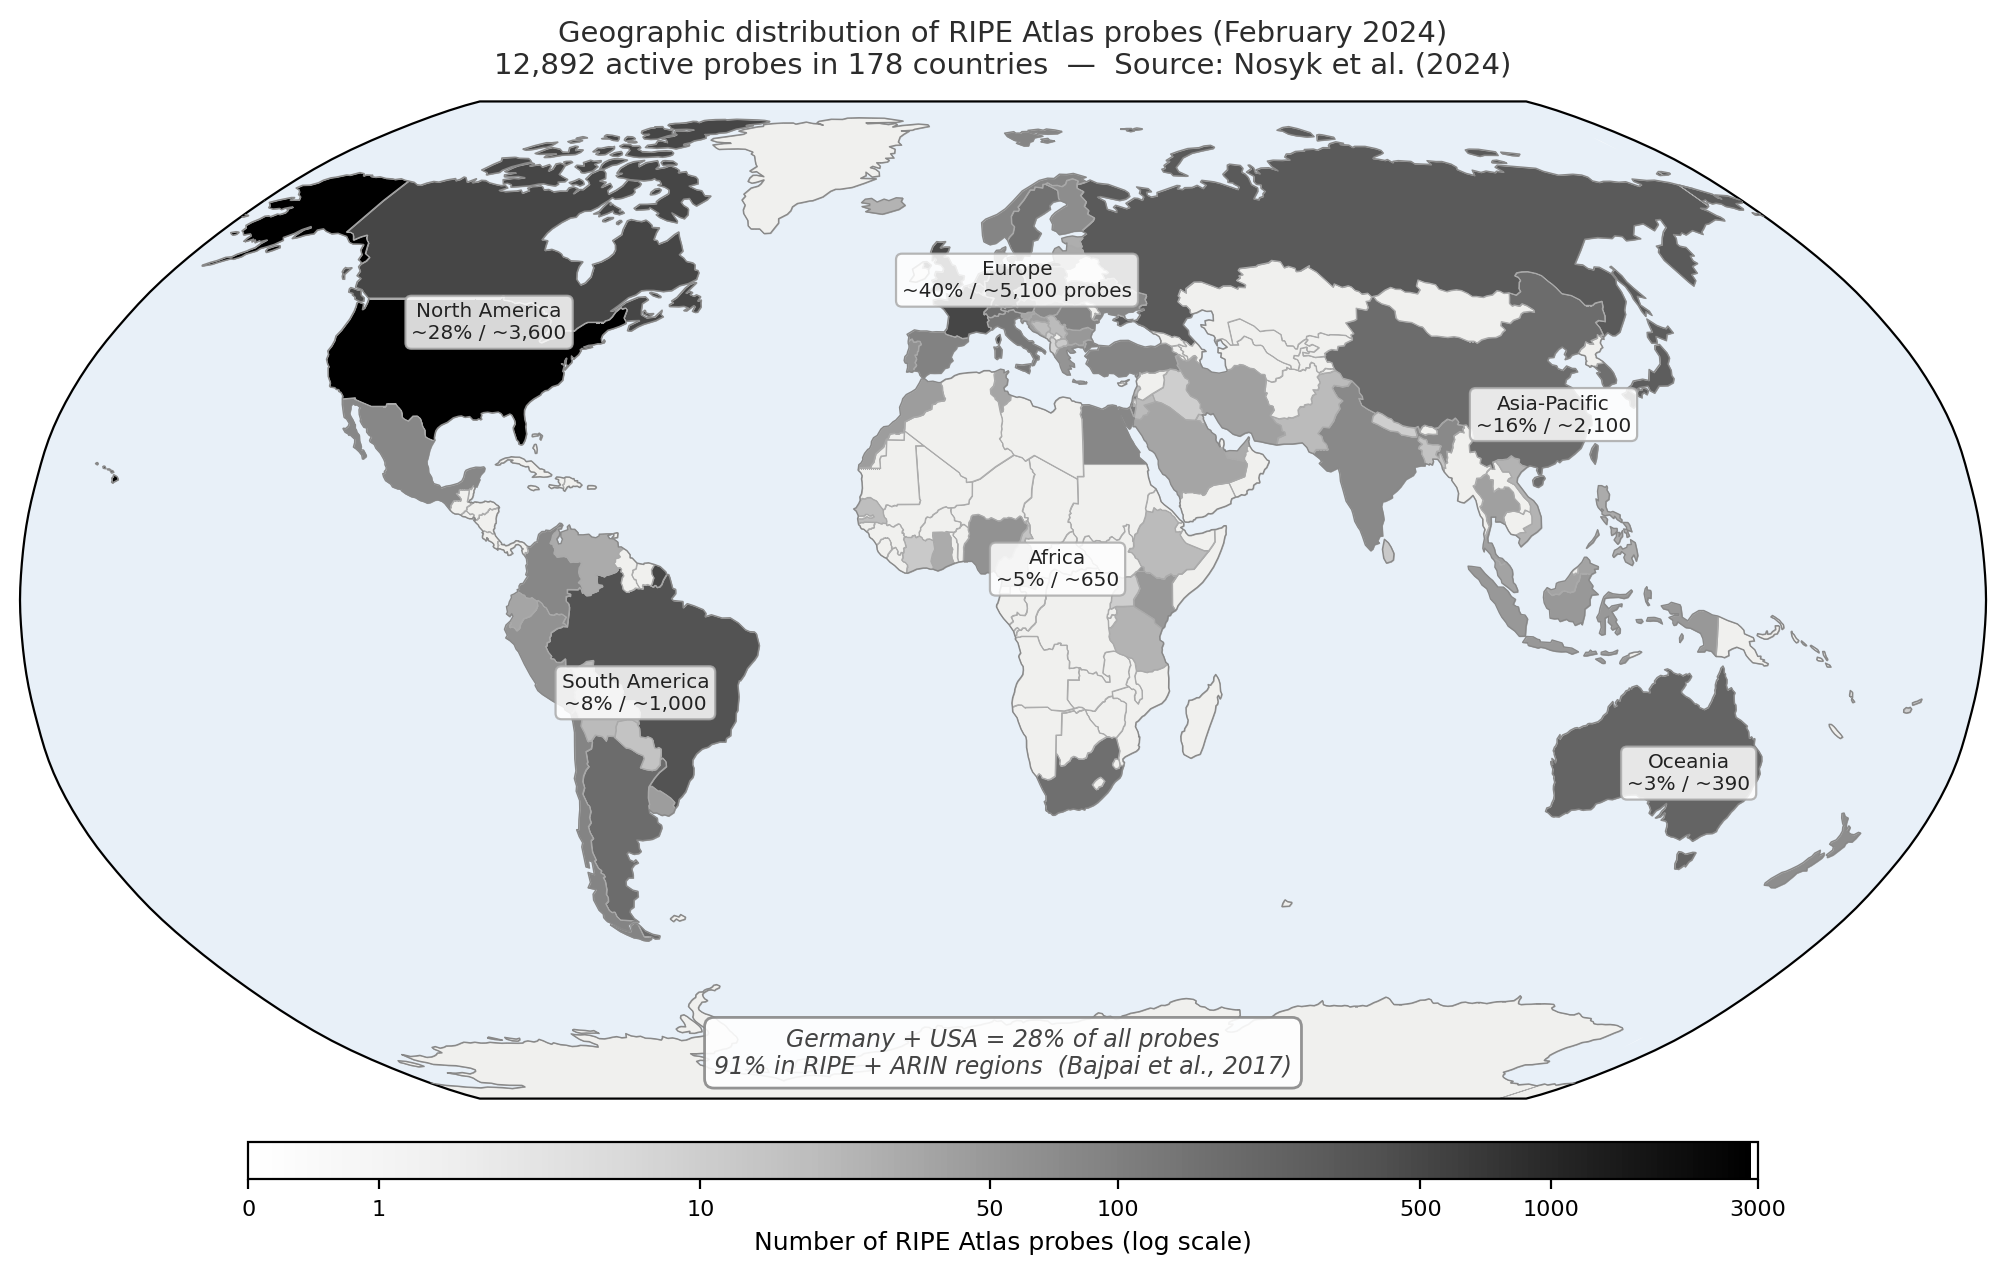
\includegraphics[width=0.90\linewidth]{figures/fig4_ripe_atlas_distribution.png}
  \caption{Geographic distribution of RIPE Atlas probes (February 2024). Choropleth on a Robinson projection; probe counts per country on a logarithmic scale. Germany and the USA together account for 28\% of all active probes; 91\% of dual-stacked probes are concentrated in the RIPE (Europe/Middle East) and ARIN (North America) regions~\cite{Bajpai2017,Nosyk2024}. Country probe counts are approximate, derived from published regional statistics.}
  \label{fig:ripe_atlas_distribution}
\end{figure}

\textbf{Measurement interference}: Holterbach et al.~\cite{Holterbach2015} provide the definitive empirical characterisation of interference between concurrent measurements on RIPE Atlas. The platform schedules measurements from multiple users concurrently on the same probes, which creates two forms of interference. First, \textbf{precision degradation}: when a probe is under concurrent measurement load, timing measurements increase by more than 1 ms in the median case and more than 7 ms at the 95th percentile, even for the newer, more powerful v3 probe hardware. Second, \textbf{temporal desynchronisation}: measurements launched nominally simultaneously from multiple probes can complete up to \textbf{one hour apart} under heavy concurrent load. Critically, Holterbach et al.~\cite{Holterbach2015} show that upgrading probe hardware reduces precision degradation but does not resolve desynchronisation --- the latter is a scheduling and network propagation problem, not a computation problem. The authors further demonstrate that historic RIPE Atlas datasets may have been affected by interference, and recommend two mitigation strategies: scheduling measurements at off-peak periods to reduce concurrent load, and using multiple repeated measurements to identify interference-induced outliers.
\bigskip
\section{Anycast Routing in the DNS Infrastructure}
\label{sec:2.5}

IP anycast is the dominant routing architecture for DNS root servers, TLD servers, large public resolvers (Google 8.8.8.8, Cloudflare 1.1.1.1), and many authoritative name servers. Understanding anycast --- and its implications for geographic routing variation --- is essential context for interpreting distributed DNS measurements: probes at different geographic locations may contact physically different servers behind the same anycast IP address, and the resulting DNS responses may differ not only in which IP is returned, but in response latency and even content.

\subsection{Internet-Wide Anycast Deployment}
\label{subsec:2.5.1}

Cicalese et al.~\cite{Cicalese2015} conduct the first Internet-wide census of IPv4 anycast adoption, scanning the entire routable IPv4 address space from approximately 300 PlanetLab vantage points spread across research institutions. The detection principle is the \textbf{speed-of-light constraint}: if two geographically separated vantage points observe round-trip times to the same IP address that are inconsistent with a single physical server --- that is, the latency "disks" (circles of radius RTT/2 centred on each VP) do not intersect --- the target must be anycast, with each VP contacting a different replica.

Anycast replica enumeration uses the \textbf{Maximum Independent Set} (MIS) algorithm on the set of non-overlapping latency disks, which conservatively lower-bounds the number of distinct replicas. Geolocation of each replica applies a maximum-likelihood estimator biased toward city population within the smallest bounding latency disk, validated against known CDN ground truths (Cloudflare, Edgecast). Cicalese et al.~\cite{Cicalese2015} report approximately 75\% city-level accuracy with a median geolocation error of 350 km for incorrectly located replicas.

Key census findings: approximately \textbf{10\textasciicircum{}3 IPv4 /24 subnets} are anycast in the current Internet; each deployment serves on average approximately \textbf{10 replicas} (a conservative lower bound given the 300-VP limitation); anycast is used not only by DNS operators but by tier-1 ISPs, CDNs, cloud providers, network equipment vendors, and DDoS mitigation services. Cicalese et al.~\cite{Cicalese2015} note an important calibration result for the thesis: studies targeting individual anycast deployments (e.g., DNS root servers) use O(10\textasciicircum{}4)--O(10\textasciicircum{}5) vantage points to achieve approximately 90\% replica recall --- a figure that motivates the use of RIPE Atlas's 12,000+ probes for high-recall anycast characterisation.

\subsection{Anycast Instance Identification Techniques}
\label{subsec:2.5.2}

Two complementary techniques allow active DNS measurements to identify which physical anycast instance responded to a query, without requiring access to BGP routing tables:

\textbf{NSID option (RFC 5001)}: The NSID EDNS option is appended to a DNS query in the OPT record's Additional section. The responding server includes a server-defined identifier string in the OPT record of its response. The NSID string typically encodes the instance's location (e.g., \texttt{dns.th2.nic.fr} for the Paris instance of d.nic.fr, \texttt{dns.fra.nic.fr} for Frankfurt). NSID can be added to any DNS query type (A, AAAA, SOA, etc.), making it universally applicable to any anycast service that implements it. Bortzmeyer~\cite{Bortzmeyer2013} uses NSID to characterise the instance distribution of d.nic.fr across approximately 500 RIPE Atlas probes in six measurement runs.

\textbf{"id.server" CHAOS query (RFC 4892)}: Querying for \texttt{id.server} in the DNS CHAOS class (\texttt{TXT id.server CHAOS}) returns a text string identifying the responding instance --- typically an IATA airport code (e.g., \texttt{ams} for Amsterdam, \texttt{fra} for Frankfurt) or a city abbreviation. CHAOS class records are not cached by resolvers, because the CHAOS class is outside the normal IN (Internet) class caching scope, guaranteeing that each query reaches the actual BGP-routed anycast instance rather than a cached response from a different resolution path. Finnegan~\cite{Finnegan2018} identifies this cache-bypassing property as the mechanism's key advantage for anycast characterisation.

As Finnegan~\cite{Finnegan2018} explains, \texttt{id.server} is the preferred technique when supported by a service, since it is specifically designed for instance identification; NSID serves as the universal fallback applicable to any query type. A third complementary approach used by Edgecast (2017) is \textbf{penultimate-hop traceroute analysis}: traceroutes from the 12 RIPE Atlas anchors hosted by Edgecast are analysed for the penultimate hop (the last router hop before the CDN server), whose IP address encodes the CDN PoP identity and can be used to map the traceroute's routing path to a specific Point of Presence.

\subsection{BGP Attraction Basins and IPv4/IPv6 Divergence}
\label{subsec:2.5.3}

Two empirical findings from the anycast DNS measurement literature have direct implications for interpreting geographic DNS variation in this thesis.

\textbf{BGP attraction basins} \cite{Bortzmeyer2013,Finnegan2018}: BGP routing directs each anycast query to the "nearest" replica in BGP path-length terms, where "nearest" is determined by the AS-path topology of peering agreements and transit relationships --- not by geographic proximity. Bortzmeyer~\cite{Bortzmeyer2013} demonstrates this counter-intuitive effect strikingly for d.nic.fr, the \textit{.fr} TLD's anycast authoritative name server: in IPv4, the \textbf{Paris instance} (dns.th2.nic.fr) and the \textbf{Frankfurt instance} (dns.fra.nic.fr) each attract approximately \textbf{36\% of global queries}. But North American probes route \textbf{55\% of their traffic to Paris} and only 33\% to Frankfurt --- despite Paris being approximately 6,000 km farther from North America than a theoretically well-placed US instance would be. Asia-Pacific probes similarly route approximately 38\% to Paris. This pattern reflects BGP peering arrangements that make European PoPs the BGP-shortest path for large portions of non-European network space --- a phenomenon Bortzmeyer~\cite{Bortzmeyer2013} terms "BGP attraction basins."

Finnegan~\cite{Finnegan2018} confirms the same pattern at operational scale for UncensoredDNS: 500 RIPE Atlas probes (250 globally distributed, 250 US-focused) reveal strong European coverage but very limited US West Coast presence, identified as a gap that a Fremont Internet Exchange Point PoP would address. The 250/250 probe split strategy --- a global component for worldwide distribution characterisation plus a region-focused component for fine-grained regional analysis --- is directly applicable to the measurement design of this thesis. Figure~\ref{fig:bgp_attraction_basins} depicts the BGP attraction basins documented by Bortzmeyer~\cite{Bortzmeyer2013} for d.nic.fr.

\begin{figure}[tp]
  \centering
  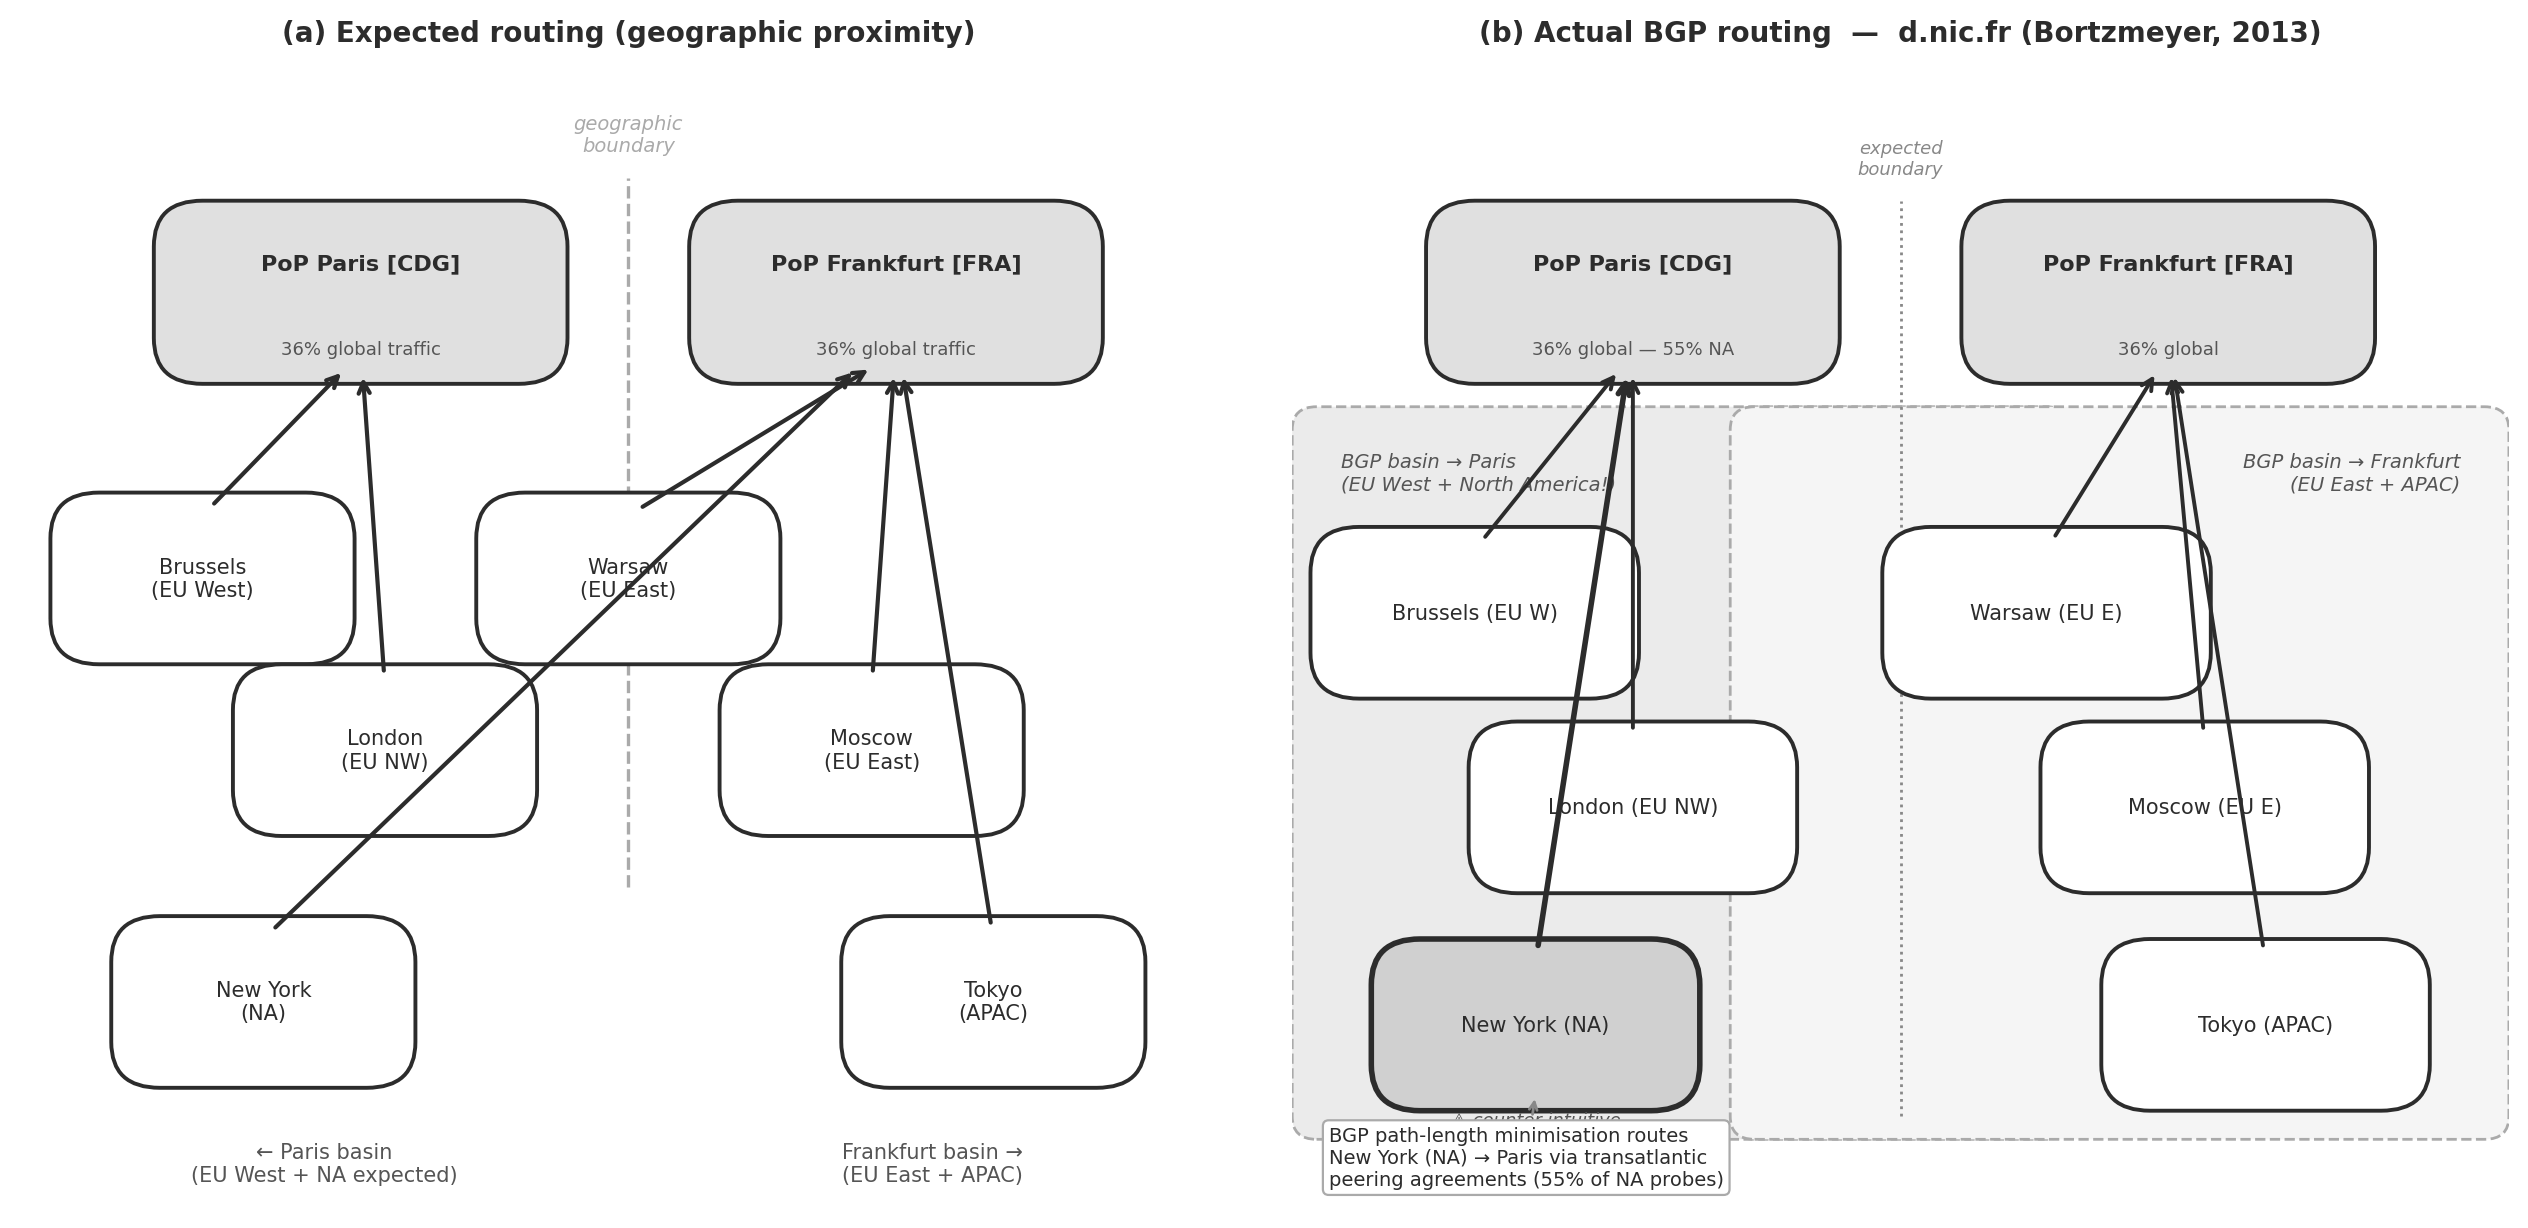
\includegraphics[width=0.92\linewidth]{figures/fig6_bgp_attraction_basins.png}
  \caption{BGP attraction basins in anycast DNS routing, illustrated for d.nic.fr~\cite{Bortzmeyer2013}. \textbf{(a) Expected routing}: geographic proximity would route EU West clients to Paris and EU East / APAC clients to Frankfurt. \textbf{(b) Actual BGP routing}: North American probes route 55\% of their queries to Paris due to BGP peering arrangements, despite the ~6,000 km additional distance. BGP path-length topology, not geography, determines attraction basin boundaries.}
  \label{fig:bgp_attraction_basins}
\end{figure}

\textbf{IPv4/IPv6 anycast divergence} \cite{Bortzmeyer2013}: The IPv4 and IPv6 BGP routing tables are maintained independently; they may propagate different prefixes and reflect different peering relationships for the same anycast service. Bortzmeyer~\cite{Bortzmeyer2013} documents a striking reversal for d.nic.fr: the dominant instance \textbf{reverses between protocols} --- Frankfurt receives \textbf{36\% of global IPv6 queries} (dominant) but only 17\% in IPv4 (subordinate); Paris receives 36\% in IPv4 but only 17\% in IPv6. This result demonstrates that dual-stack measurements must be run and analysed separately: combining IPv4 and IPv6 probes in a single analysis would obscure a qualitative difference in anycast routing.

For CDN PoP optimisation, Edgecast (2017) test six different probe grouping strategies --- by country, by geolocation, by ASN, by RIR region, by continent, and by clustering --- and find that \textbf{geolocation-based grouping} provides the best trade-off between routing accuracy and interpretability. They also propose a logistic-normalised scoring framework (+1 for improved routing, -1 for degraded routing) that quantifies the net impact of anycast BGP configuration changes on per-PoP traffic distribution across probe groups. This scoring framework is adaptable to this thesis's analysis of geographic DNS response variation.

\subsection{Anycast Routing Quality and Application Context}
\label{subsec:2.5.4}

The performance cost of BGP-based anycast routing --- its potential to deliver clients to geographically or topologically suboptimal replicas --- was systematically quantified by Koch et al.~\cite{Koch2021} in the largest comparative study of anycast inflation to date, covering both the DNS root server system and Microsoft's global CDN.

Koch et al.~\cite{Koch2021} distinguish \textbf{geographic inflation} (the assigned replica is farther than the closest deployed site) from \textbf{latency inflation} (the measured RTT exceeds the theoretical minimum from the closest site). For root DNS, they find that more than \textbf{95\% of users} experience some geographic inflation for at least one root letter, and up to 40\% experience more than 100 ms of inflation to individual root letters. However, when averaged across all root letters --- exploiting the fact that recursive resolvers preferentially route queries to their best-performing letter among the 13 root addresses --- only \textbf{10\% of users} experience more than 100 ms of inflation.

Critically, Koch et al.~\cite{Koch2021} argue that root DNS inflation is \textbf{practically irrelevant to users}. Root DNS records have TTLs of approximately 518,400 seconds (six days), meaning recursive resolvers contact the root DNS at most once per root record per six days. The additional latency from inflation is amortised across thousands of queries served from cache, making its per-user-query cost negligible. By contrast, Microsoft's CDN serves directly user-facing content where each HTTP connection involves multiple RTTs to the front-end server. Here, inflation directly degrades user experience: the authors estimate that if Microsoft's CDN suffered the same inflation as individual root letters, each page load would incur hundreds of additional milliseconds. Microsoft has therefore invested heavily in peering agreements to limit CDN inflation to approximately \textbf{35\% of users experiencing any inflation}.

For this thesis, these findings provide important context for interpreting DNS timing variations across RIPE Atlas probes. Observed RTT differences between probes querying the same anycast DNS server do not necessarily reflect the geographic routing variation relevant to DNS response content --- the IP address returned in the A record. The routing of the DNS query (which anycast instance answers) may differ from the routing of subsequent data connections to the IP address returned. Both dimensions require separate characterisation.

Koch et al.~\cite{Koch2021} use RIPE Atlas directly in their study: 7,000 ping measurements from 1,000 probes (3 measurements per probe per CDN ring) serve as supplementary calibration data for the CDN latency analysis, illustrating how RIPE Atlas can complement server-side logs to provide client-perspective ground truth.
\bigskip
\section{Content Delivery Networks and DNS-Based Geographic Routing}
\label{sec:2.6}

CDNs distribute content across geographically dispersed server clusters and use DNS as the primary mechanism to direct each client to an appropriate replica. The interaction between DNS resolution and CDN routing is central to our thesis: understanding it explains why different geographic vantage points may receive different DNS responses for the same domain, and what those differences mean in terms of content accessibility.

\subsection{DNS as the Dominant CDN Redirection Mechanism}
\label{subsec:2.6.1}

Wang et al.~\cite{Wang2018} provide a systematic survey of DNS-based CDN server redirection, positioning it as "the most popular means of deploying CDNs" due to its compatibility with existing DNS infrastructure and ease of deployment without requiring client-side software changes. The CDN request routing problem involves two sub-problems: a \textbf{server selection mechanism} (choosing the optimal replica based on network distance, server load, latency, and availability) and a \textbf{server redirection mechanism} (directing the client to the selected replica). DNS-based redirection uses the DNS resolution process as the redirection channel: the CDN's authoritative name server returns a different A/AAAA record or CNAME depending on the inferred location of the querying resolver. Major CDNs using this approach include Akamai (which pioneered DNS-based CDN redirection), Limelight Networks, and Mirror Image \cite{Wang2018}.

Calder et al.~\cite{Calder2015} empirically evaluate a production anycast CDN --- Microsoft's Bing front-end network --- and find that anycast-based redirection (where BGP routing, rather than DNS, directs clients to replicas) directs approximately \textbf{20\% of clients to suboptimal front-end servers} relative to the geographically closest available front-end. For this 20\% of affected clients, switching to DNS-based unicast redirection --- where a geolocation-aware DNS system selects the closest front-end server and returns its IP directly --- could improve latency by \textbf{7 to 100 ms} depending on the client's region and routing context. This result confirms that BGP's performance-agnostic routing creates measurable quality-of-service degradation even at a well-engineered commercial CDN, and motivates the hybrid DNS-anycast architectures adopted by major CDNs: anycast for proximity and resilience, DNS for fine-grained routing corrections. To investigate the causes, Calder et al.~\cite{Calder2015} use RIPE Atlas traceroutes as a diagnostic complement to server-side logs and JavaScript beacon measurements --- illustrating the platform's role as a flexible supplementary measurement tool for validating client-perspective routing hypotheses derived from server-side data. The geographic distribution of the 20\% suboptimal clients is non-uniform: clients in regions where Bing operates few anycast PoPs (e.g., parts of South America, Africa, and Southeast Asia) experience higher inflation rates than clients in densely covered regions (North America, Western Europe). This geographic heterogeneity in anycast routing quality parallels the heterogeneity in DNS response geography that this thesis sets out to characterise.

Li et al. (2025), studying Twitch's global CDN for live video streaming, find that DNS-based CDN routing for Twitch operates at \textbf{continent-level granularity}: distinct groups of CDN server IP addresses are assigned to clients in Europe, North America, Asia-Pacific, and other regions, with the assignment determined by the querying resolver's inferred continent. This coarse geographic partitioning simplifies CDN management but creates sharp geographic boundaries in DNS response content --- boundaries detectable through distributed active measurement.

\subsection{The Remote DNS Problem}
\label{subsec:2.6.2}

DNS-based CDN routing critically assumes that the recursive resolver's IP address is a reliable proxy for the end user's geographic location --- specifically, that the resolver is topologically close to its clients. Wang et al.~\cite{Wang2018} identify the \textbf{remote DNS problem}: this assumption fails when clients use a centralised public resolver (Google 8.8.8.8, Cloudflare 1.1.1.1, OpenDNS) that is geographically or topologically distant from the client. When the CDN authoritative server receives a DNS query from a public resolver in California, it may return a California-optimised CDN replica even though the actual client is in Brazil. The result is suboptimal server assignment and degraded content delivery performance.

Hours et al.~\cite{Hours2016} quantify this effect causally using passive TCP traffic traces from a large European ISP and a Bayesian causal network (PC algorithm + do-calculus). Their analysis confirms a causal pathway: clients using \textbf{Google DNS} (GDNS) are assigned geographically farther Akamai CDN servers than equivalent clients using their \textbf{local ISP DNS} (LDNS), resulting in higher ISP-side RTT and reduced download throughput. A secondary finding --- not predictable from correlation analysis alone --- is that servers assigned to GDNS users are configured with a smaller TCP initial congestion window than servers assigned to LDNS users, amplifying the throughput difference beyond the server-distance effect.

Wang et al.~\cite{Wang2018} quantify the scale of the remote DNS problem: public DNS service adoption among Internet users is growing at approximately \textbf{27\% per year}, meaning that a rapidly increasing fraction of DNS queries to CDN authoritative servers originate from a small number of centralised resolver IP addresses rather than the diverse set of ISP resolvers that would accurately reflect client geography. The study measures this as a distance mismatch between the CDN server assigned by the remote resolver and the CDN server geographically closest to the actual client, finding mismatches of up to \textbf{113\%} --- meaning the assigned server is more than twice as far as the optimal server. At these mismatch levels, the impact on throughput and latency is measurable even for users with high-bandwidth connections. Wang et al.~\cite{Wang2018} frame this as the "remote DNS paradox": the very features that make public DNS services popular with users (reliability, performance, privacy) are precisely the features that degrade CDN routing quality, because those features require operating a centralised resolver fleet rather than a geographically distributed one. Hours et al.~\cite{Hours2016} confirm the causality of this effect for the Akamai CDN from the perspective of a large French ISP: clients using Google DNS are assigned servers that are, on average, \textbf{20 ms farther} in RTT than servers assigned to equivalent clients using the ISP's own resolver, with a secondary server configuration effect that reduces download throughput by approximately \textbf{14\%}.

The remote DNS problem is directly relevant to RIPE Atlas measurements: probes that use a public resolver (rather than their local ISP resolver) will obtain CDN-assigned IP addresses based on the public resolver's location, not the probe's location. This must be accounted for when interpreting geographic variation in DNS A/AAAA responses across probes with heterogeneous resolver configurations.

\subsection{EDNS Client Subnet: Mechanism, Deployment, and Privacy Trade-offs}
\label{subsec:2.6.3}

The \textbf{EDNS Client Subnet} (ECS) extension, specified in RFC\textasciitilde{}7871~\cite{RFC7871}, addresses the remote DNS problem by embedding a truncated version of the client's IP address in the DNS query forwarded from the recursive resolver to the authoritative CDN name server. The ECS EDNS option carries four fields:

\begin{itemize}
  \item \textbf{FAMILY}: Address family (1 = IPv4, 2 = IPv6).
  \item \textbf{SOURCE PREFIX-LENGTH}: The number of bits of the client address included in the option. RFC\textasciitilde{}7871~\cite{RFC7871} recommends /24 for IPv4 and /48 for IPv6, balancing geographic precision with privacy protection.
  \item \textbf{SCOPE PREFIX-LENGTH}: Set by the authoritative server in the response; indicates how many bits of the client address were actually used in selecting the response. A scope of /0 means the response applies globally and is not location-specific.
  \item \textbf{ADDRESS}: The truncated client IP prefix.
\end{itemize}

An ECS-aware CDN authoritative server uses the ADDRESS field --- the client's IP prefix --- rather than the resolver's source IP to select the appropriate CDN replica, then returns the SCOPE in the response. Intermediate caches must store separate entries keyed by (question, ECS scope prefix), since the same domain may resolve differently for clients in different /24 subnets. This \textbf{per-scope caching} inflates resolver cache size substantially, a concern acknowledged in RFC\textasciitilde{}7871~\cite{RFC7871} but not quantified.

ECS introduces a fundamental privacy trade-off (Wang et al., 2018; RFC\textasciitilde{}7871~\cite{RFC7871}): forwarding the client's IP prefix to the authoritative CDN server --- and to any on-path observer --- makes the client's network location visible to infrastructure that would otherwise only see the resolver's IP. RFC\textasciitilde{}7871~\cite{RFC7871} explicitly acknowledges this: "if we were just beginning to design this mechanism, and not documenting existing protocol, it is unlikely that we would have done things exactly this way." The RFC recommends that ECS be \textbf{disabled by default} and enabled only when the performance benefit is clear. A further privacy risk identified by Wang et al.~\cite{Wang2018} is \textbf{redirection enumeration}: an adversary with ECS-enabled queries can systematically probe the CDN's mapping from client IP prefixes to server assignments, exposing the CDN's traffic engineering policies.

For RIPE Atlas measurements, the practical deployment of ECS is limited. Bortzmeyer~\cite{Bortzmeyer_tutorial} reports that a test of 100 Belgian Atlas probes found that only a small number used resolvers that forwarded ECS options. This means that, for most probes, the DNS response is determined by the resolver's IP address (the pre-ECS default behaviour) rather than the probe's IP. Researchers wishing to disable ECS explicitly --- to obtain resolver-IP-determined responses consistently --- can include an ECS option with SOURCE PREFIX-LENGTH = 0 in their queries; Google Public DNS, for instance, respects this opt-out (Bortzmeyer, n.d., tutorial). Figure~\ref{fig:ecs_schema} illustrates the three ECS scenarios.

\begin{figure}[tp]
  \centering
  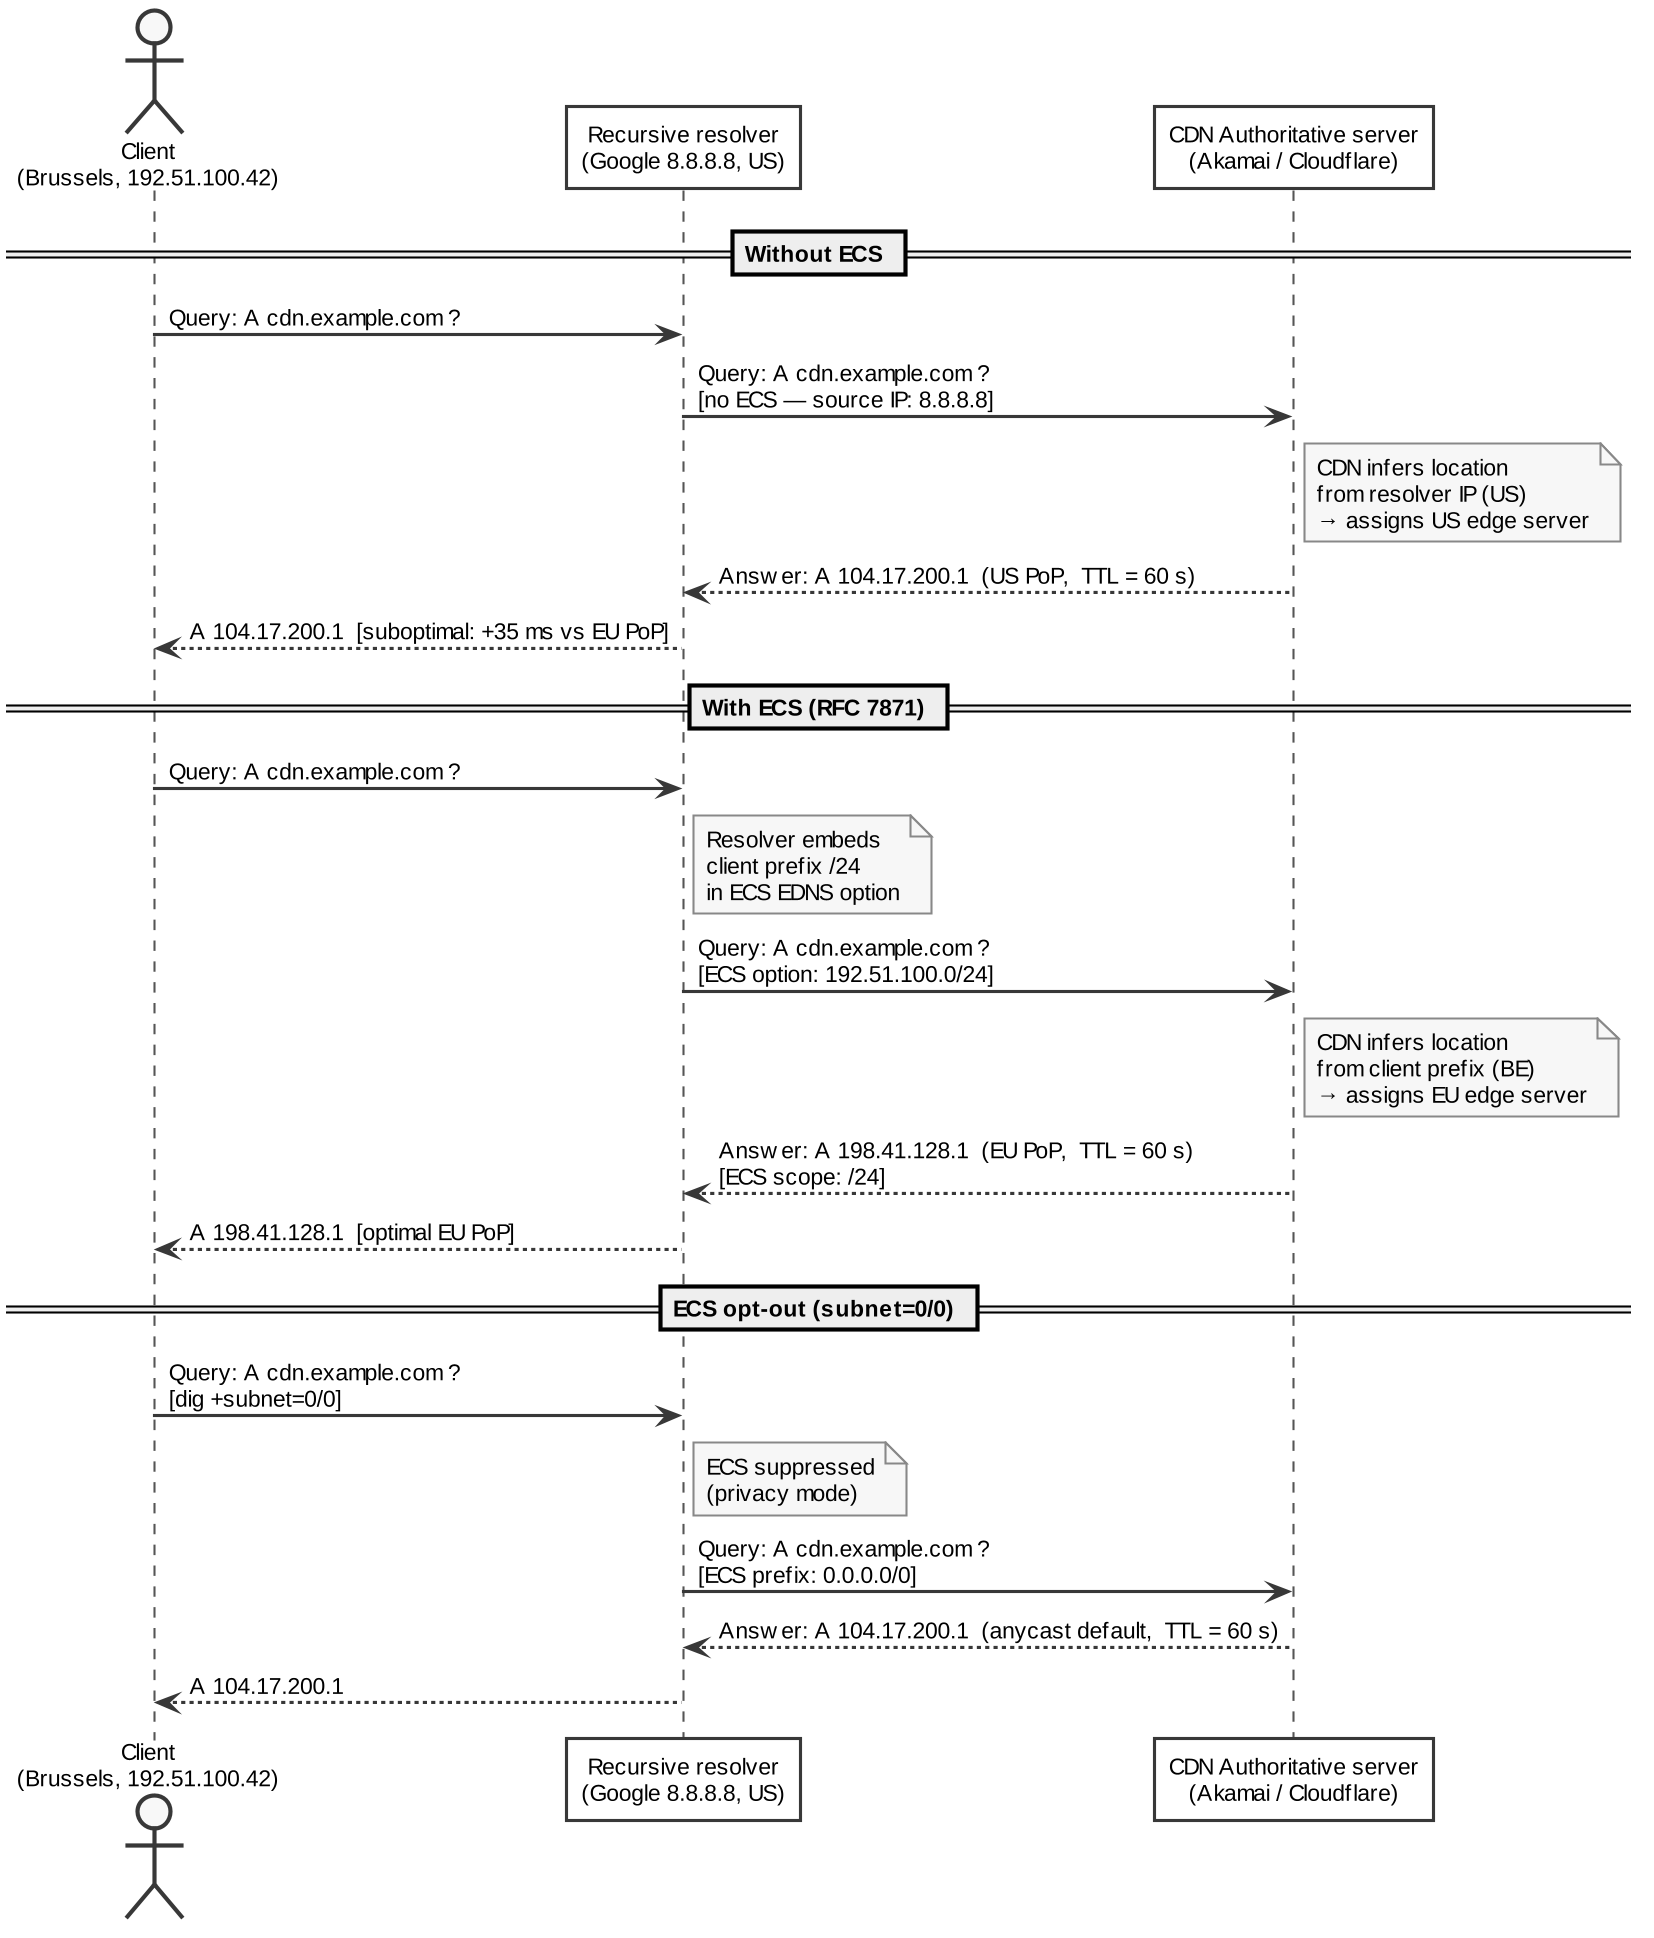
\includegraphics[width=0.90\linewidth]{figures/fig5_ecs_schema.png}
  \caption{Effect of EDNS Client Subnet (ECS, RFC\protect~7871) on CDN geographic routing. \textit{Without ECS}, the CDN authoritative server infers client location from the recursive resolver's IP (8.8.8.8, US), assigning a suboptimal US edge server to a Belgian client. \textit{With ECS}, the resolver embeds the client's /24 prefix; the CDN selects the geographically appropriate EU PoP. \textit{ECS opt-out} (\texttt{subnet=0/0}) suppresses the prefix entirely, reverting to resolver-IP-based routing.}
  \label{fig:ecs_schema}
\end{figure}

\subsection{Alternative Solutions to the Remote DNS Problem}
\label{subsec:2.6.4}

Wang et al.~\cite{Wang2018} catalogue and compare three main approaches to the remote DNS problem, each with different deployment complexity, privacy implications, and effectiveness:

\textbf{ECS (EDNS Client Subnet)}: Described above. Effective for CDNs that implement it; major performance benefit over plain remote DNS; significant privacy cost; caching complexity; not universally deployed. Wang et al.~\cite{Wang2018} note that ECS is a "recognised solution" but its privacy cost and the conditional deployment recommendation of RFC\textasciitilde{}7871~\cite{RFC7871} limit its reach.

\textbf{Name extension}: The client's IP address prefix is encoded in the domain name itself --- for example, \texttt{<client-prefix>.cdn.example.com} --- and the CDN authoritative server selects a response based on the prefix encoded in the queried name. This approach avoids the ECS privacy problem (the prefix is visible in the query name, not in an EDNS option, but both are observable) and does not require EDNS support. However, it requires the recursive resolver to forward the original query name unmodified, and it inflates the DNS namespace with per-prefix subdomains, complicating zone management.

\textbf{Direct resolution}: The client bypasses recursive resolvers entirely and contacts the CDN authoritative server directly, or the CDN provides a resolver co-located with its edge servers. This eliminates the LDNS-client distance problem at the cost of losing resolver-level privacy protection, requiring client software changes, and potentially exposing the client's IP directly to the CDN operator. Wang et al.~\cite{Wang2018} consider this approach impractical for general deployment, though it is implemented in specialised scenarios (e.g., mobile CDN clients that contact CDN-provided resolvers).

For this thesis, the implication of this landscape is that no single DNS measurement protocol can capture all aspects of CDN routing: ECS-enabled queries may return CDN-assigned addresses different from those returned by non-ECS queries for the same probe. Controlling for ECS behaviour --- by either consistently disabling ECS (subnet=0/0) or consistently enabling it at /24 granularity --- is an important measurement design choice documented in Chapter 4.
\bigskip
\section{Domain Ranking Lists: From Alexa to Tranco}
\label{sec:2.7}

Studies of DNS behaviour at scale require a representative and reproducible corpus of domain names. The choice of domain list has significant implications for result validity, research reproducibility, and resistance to adversarial manipulation.

\subsection{Problems with Commercial Ranking Lists}
\label{subsec:2.7.1}

Le Pochat et al.~\cite{LePochat2019} systematically evaluate the four main freely available domain ranking lists across five properties: similarity, stability, representativeness, responsiveness, and benignness. The four lists analysed are \textbf{Alexa} (Amazon subsidiary, based on browser extension traffic), \textbf{Cisco Umbrella} (based on DNS traffic to OpenDNS), \textbf{Majestic} (based on web crawl backlinks), and \textbf{Quantcast} (based on US-centric traffic instrumentation).

\textbf{Similarity}: Despite all four lists purporting to rank "the most popular domains on the Internet", they agree on only approximately 70,000 domains out of a combined pool of \textasciitilde{}2.82 million unique domains. The rank-biased overlap (RBO) --- a similarity measure that weights highly-ranked domains more heavily --- remains between 24\% and 33\% even when the top 100 domains receive most of the weight. This means that choosing Alexa rather than Umbrella for a study of the top 10,000 domains yields a substantially different set of domains, potentially changing study conclusions \cite{LePochat2019}.

\textbf{Stability}: Majestic's list changes by at most 1\% per day, making it the most stable. Cisco Umbrella changes by approximately 10\% daily. Alexa, which was similarly stable to Majestic through January 2018, underwent an undisclosed change in its averaging methodology that caused daily turnover to reach approximately \textbf{50\% of the list} --- meaning half the domains on Alexa's "top million" change every day. This extreme volatility makes Alexa-based longitudinal studies unreliable, since the domain corpus changes faster than the phenomena being studied.

\textbf{Representativeness and benignness}: Cisco Umbrella includes approximately 51\% entries that are not actual web domains --- EC2 internal hostnames, typo domains (e.g., \texttt{google.conm}), and internal corporate names that happen to be visible in OpenDNS query traffic. Majestic's list, widely used as a whitelist, contains 2,162 malicious domains --- a dangerous characteristic for security research that treats list membership as an indicator of legitimacy.

\textbf{Manipulability}: Le Pochat et al.~\cite{LePochat2019} empirically demonstrate that every list has at least one low-cost manipulation technique. The most striking finding is that \textbf{a single HTTP request from a browser with the Alexa extension} suffices to increment a domain's request count for that day --- and the authors experimentally reach a rank as good as \textbf{28,798} with minimal effort. For Cisco Umbrella, injecting DNS queries from a single recursive resolver that participates in the Umbrella data collection suffices to inflate a domain's apparent popularity. For Majestic, creating links from a small set of domains already in the Majestic index is sufficient. Le Pochat et al.~\cite{LePochat2019} note that none of the commercial list operators publishes the full details of their ranking methodology, making it impossible to audit the lists for manipulation or to reproduce their ranking calculations independently. This opacity is not merely an academic concern: security researchers who use these lists as whitelists (treating top-ranked domains as legitimate) are exposed to adversarial list manipulation; and researchers who compare results across studies may be comparing datasets whose domain compositions differ substantially due to methodology differences rather than actual changes in Internet usage. The security dimension is particularly acute: van der Toorn et al.~\cite{vanderToorn2018} note that malicious actors have strong incentives to inflate their domains' ranks on traffic-based lists, since a high rank provides social legitimacy. This makes Alexa trivially manipulable by adversaries seeking to insert malicious domains into whitelists or to bias research results toward domains they control. Table~\ref{tab:ranking_lists} compares the four lists across the key properties identified by Le~Pochat et al.~\cite{LePochat2019}.

\begin{table}[H]
\centering
\small
\begin{tabularx}{\linewidth}{p{2.2cm} X X X X}
\toprule
\textbf{Property} & \textbf{Alexa} & \textbf{Cisco Umbrella} & \textbf{Majestic} & \textbf{Tranco} \\
\midrule
Data source       & Browser extension traffic & DNS queries to OpenDNS & Web crawl backlinks & Multi-source aggregation \\
Daily change rate & $\approx$50\% (post-2018) & $\approx$10\%           & $\approx$1\%        & $\approx$0.6\% \\
Manipulation effort & 1 HTTP request from browser ext. & 1 DNS query injection & Few backlinks from indexed domains & 4$\times$ effort vs.\ single-source lists \\
Non-domain entries & Low                       & $\approx$51\% (EC2 hostnames, typos…) & Low              & Filtered (HTTP 200 + safe browsing) \\
Malicious domains & Some                      & Some                  & 2,162 documented  & Filtered \\
Reproducibility   & Daily overwrite (no archive) & Daily overwrite     & Daily overwrite   & Stable permalink per list version \\
Recommended for   & Legacy reference only     & DNS-traffic studies (with caution) & Backlink analysis & DNS/security research \\
\bottomrule
\end{tabularx}
\caption{Comparison of freely available domain ranking lists. Stability, manipulation resistance, and reproducibility data from Le~Pochat et al.~\cite{LePochat2019}. Tranco is the only list designed with research reproducibility and manipulation resistance as explicit objectives.}
\label{tab:ranking_lists}
\end{table}

\subsection{Tranco: Aggregation, Stability, and Manipulation Resistance}
\label{subsec:2.7.2}

Le Pochat et al.~\cite{LePochat2019} propose \textbf{Tranco} as a research-oriented alternative that addresses all four identified limitations. Tranco is publicly available at \url{https://tranco-list.eu} and operates as follows:

\textbf{Multi-source aggregation}: Tranco aggregates multiple ranking lists --- originally Alexa, Cisco Umbrella, Majestic, and Quantcast --- using either the \textbf{Borda count} or the \textbf{Dowdall rule}. In the Borda count, each domain receives a score equal to N - rank\_i for each list where it appears (N is the maximum rank considered; rank\_i is the domain's rank in list i), and scores are summed across lists. The Dowdall rule assigns a score of 1/rank\_i per list. Both methods give higher weight to domains that rank highly across multiple lists, and assign nonzero scores to domains absent from some lists (based on their worst-case rank). Aggregation across multiple data sources reduces the influence of any single source's biases and requires that an adversary manipulate multiple independent lists to affect Tranco rankings.

\textbf{Temporal smoothing}: Aggregation is performed over a \textbf{30-day rolling window} of daily list snapshots. Each domain's rank is derived from the aggregated scores over these 30 days, smoothing out day-to-day volatility. The result: Tranco changes by only \textbf{0.6\% per day} (versus \textasciitilde{}50\% for Alexa), providing a stable corpus for longitudinal studies.

\textbf{Manipulation resistance}: Because an adversary must manipulate multiple lists over 30 days to shift a Tranco ranking, Le Pochat et al.~\cite{LePochat2019} show that manipulating Tranco to achieve the same rank as in existing lists requires at least \textbf{quadrupled effort}.

\textbf{Reproducibility}: Historical Tranco lists are archived and accessible via a stable URL including the list generation parameters. A researcher can retrieve the exact list version used in a previous study, enabling reproduction and replication of results --- a fundamental requirement of scientific research that commercial lists cannot guarantee (they overwrite their previous version daily).

For this thesis, Tranco is the appropriate choice for the domain corpus: stability ensures that the same set of domains is measured across multiple campaign repetitions, enabling meaningful temporal comparison; manipulation resistance limits the risk that adversarially placed domains distort the DNS measurement results; and archive access supports reproducibility of the measurement dataset.
\bigskip
\section{DNS Infrastructure Centralization}
\label{sec:2.8}

Despite its designed-in distributed architecture, the DNS ecosystem has undergone progressive centralization driven by commercial consolidation and economies of scale. Xu et al.~\cite{Xu2023} provide the most comprehensive recent characterisation of this phenomenon, revealing concentration levels that are not visible from DNS query counts or market share statistics alone.

\subsection{Client-Side Resolver Centralization}
\label{subsec:2.8.1}

Xu et al.~\cite{Xu2023} introduce the \textbf{NS chain reflection} technique: a crafted DNS query sequence that causes resolvers to reveal their internal resolution chain through the sequence of NS referrals they generate at the authoritative level. Unlike the CNAME-based resolver pool discovery method proposed by Schomp et al. --- which Xu et al.~\cite{Xu2023} show is no longer effective against modern resolver architectures --- NS chain reflection works from a single vantage point and reveals the full resolver pool structure including indirect recursive resolvers.

Using this technique applied Internet-wide, Xu et al.~\cite{Xu2023} find that over \textbf{90\% of all forwarding resolvers (FDNSes)} are backed by fewer than \textbf{5\% (4,071) of indirect recursive resolvers (iRDNSes)} --- an extreme concentration in the actual DNS resolution infrastructure even when the visible surface (the set of FDNS IP addresses) appears diverse. This means that the geographic diversity of RIPE Atlas probes --- each using a different ISP resolver --- may be illusory: many of those ISP resolvers ultimately forward queries to the same small set of iRDNS clusters operated by major public DNS providers.

The practical consequence for distributed DNS measurement: querying through local resolvers provides geographic diversity in the FDNS layer but not necessarily in the resolution layer that actually contacts authoritative servers. Direct querying of authoritative servers is required to bypass this invisible centralization.

\subsection{Server-Side Authoritative DNS Centralization}
\label{subsec:2.8.2}

Analysing zone files from all 1,138 gTLDs covering 210,446,494 domain names, Xu et al.~\cite{Xu2023} find dramatic concentration on the authoritative side as well:

\begin{itemize}
  \item Just \textbf{10 DNS providers} --- operating 0.45\% (12,679) of all name servers across 1,138 gTLDs --- provide authoritative resolution for \textbf{48.5\% of all gTLD domain names}, representing over 100 million domains.
  \item More than \textbf{98\% of all domain names} rely on a \textbf{single authoritative name server provider} for all their NS records. A failure of that provider causes complete DNS unavailability for those domains.
  \item \textbf{60\% of combinations of DNS provider pairs} share underlying infrastructure, meaning enterprises that distribute their NS records across multiple providers may still implicitly share a common failure point.
\end{itemize}

The \textbf{shared infrastructure risk} is arguably more insidious than single-provider dependence. Xu et al.~\cite{Xu2023} find that 60\% of combinations of DNS provider pairs --- enterprises or domain operators who distribute their NS records across two ostensibly independent providers --- share underlying physical infrastructure. This means that a failure of a shared upstream network component (a shared transit provider, a shared IXP interconnect, or shared anycast routing infrastructure) can simultaneously affect both nominal providers, defeating the intended redundancy. Xu et al.~\cite{Xu2023} attribute this to the consolidation of Internet backbone infrastructure among a small number of global tier-1 providers, which creates hidden dependencies even among nominally independent DNS operators.

Real-world outages confirm the operational stakes: the Akamai DNS outage in June 2021, the Fastly CDN outage in June 2021, and the Facebook DNS misconfiguration in October 2021 all caused widespread Internet inaccessibility for millions of domains and users, consistent with the concentration levels documented by Xu et al.~\cite{Xu2023}. The Facebook outage of October 4, 2021 is particularly instructive from a DNS perspective: a misconfigured BGP route withdrawal caused Facebook's own authoritative name server addresses to become unreachable, making the domain unresolvable from any resolver in the world simultaneously. For a domain that relies on a single DNS provider --- which Xu et al.~\cite{Xu2023} show is over 98\% of all gTLD domains --- a provider-level BGP event of this type has no fallback. Distributed active measurement at the time of such outages can capture the propagation and recovery of DNS reachability in real time, providing empirical ground truth on outage geography and duration that server-side operator logs cannot provide from the client perspective.

For distributed DNS measurement campaigns, server-side centralization implies that measuring 10,000 Tranco domains will not yield measurements of 10,000 independent DNS infrastructures. Rather, the measurements will cluster around a small number of major DNS providers, each responding similarly for their client domains. Understanding this structure is important both for measurement design (aggregating results at provider level may be more meaningful than at domain level) and for interpreting geographic variation (variation may reflect provider-level anycast routing rather than domain-specific configuration).
\bigskip
\section{DNS Security and Measurement Validity}
\label{sec:2.9}

The integrity of DNS responses received by RIPE Atlas probes is not guaranteed: several forms of DNS manipulation can cause probes to receive responses from unexpected sources or with altered content. Three dimensions of DNS security are directly relevant to the measurement validity of this thesis.

\subsection{DNSSEC Deployment and Its Limitations}
\label{subsec:2.9.1}

DNSSEC protects the authenticity and integrity of DNS responses through a cryptographic chain of trust extending from the signed root zone (since July 2010) to individual domains. Van Rijswijk-Deij et al. (2016) include DNSKEY, DS, and RRSIG record types in the OpenINTEL standard query set specifically to monitor DNSSEC adoption at the TLD zone and domain level. The longitudinal DNSSEC study (van Rijswijk-Deij et al., USENIX Security 2017, via van Rijswijk-Deij 2018) reveals systemic key management failures: many domains that appear in signed zones suffer from expired signing keys or incomplete key rollovers, leaving them with broken DNSSEC chains that validating resolvers would reject. Bajpai et al.~\cite{Bajpai2017} note through the system tag \texttt{system-resolves-a-correctly} that DNSSEC validation is far from universal: many ISP resolvers do not validate DNSSEC signatures, passing invalid signed responses to clients without error.

For this thesis, DNSSEC matters in two ways: (1) domains with broken DNSSEC chains may return \texttt{SERVFAIL} responses from validating resolvers, which can be misidentified as measurement errors rather than security failures; and (2) DNSSEC-signed domains provide an additional data dimension for characterising the DNS infrastructure of Tranco domains. When a RIPE Atlas probe uses a validating resolver and queries a domain with a broken DNSSEC chain, the probe returns \texttt{SERVFAIL} --- the same response code returned when the authoritative server is unreachable. These two failure modes are indistinguishable without additional information. One mitigation is to include both the \texttt{DO} bit (DNSSEC OK) and the \texttt{CD} bit (Checking Disabled) in measurement queries: with \texttt{CD} set, the resolver returns the response despite DNSSEC validation failure, allowing the measurement to distinguish a DNSSEC failure (response exists with \texttt{CD} overriding validation) from a genuine unavailability (no response regardless of \texttt{CD}). Alternatively, querying authoritative servers directly --- as proposed in this thesis --- bypasses DNSSEC validation entirely, since the query is not mediated by a validating recursive resolver; the raw DNS response from the authoritative server is returned regardless of whether the DNSSEC chain is complete. This is another argument in favour of the direct-authoritative-query design choice: it eliminates both the resolver-location bias (Section 2.1.4) and DNSSEC-induced \texttt{SERVFAIL} confusion as sources of measurement artefact.

\subsection{DNS Root Manipulation and In-Path Proxies}
\label{subsec:2.9.2}

Jones et al.~\cite{Jones2016} demonstrate that DNS responses observed by RIPE Atlas probes may not originate from the expected authoritative servers. Using approximately 8,000 Atlas probes in 2,755 ASes across 189 countries, they identify ten ISPs that deploy in-path transparent DNS proxies: these proxies intercept root DNS queries from clients and answer them locally, without forwarding to the actual root servers. Detection uses two independent methods: (1) anomalous RTT --- if DNS query RTT to the B root is a factor of 23$\times$ lower than ICMP ping RTT to the same IP (14 ms vs. 318 ms for the Kenyan example), a local proxy is almost certainly involved; (2) identity mismatch --- \texttt{HOSTNAME.BIND} CHAOS queries return identifiers that do not match the expected pattern for the B root (e.g., returning the ISP's own server name rather than a B-root-consistent string).

Jones et al.~\cite{Jones2016} also find that 1.7\% of Atlas probes have inconsistent geolocation data between Atlas's own metadata and the MaxMind geolocation database, complicating latency-based detection for those probes and motivating careful probe metadata validation in any measurement campaign.

For this thesis, the DNS root manipulation findings have two implications: (1) measurement campaigns should include data quality checks (e.g., RTT sanity checks) to identify probes whose DNS responses likely originate from in-path proxies rather than the intended authoritative servers; (2) the existence of ISP-level DNS proxies means that some probes' responses reflect locally cached or filtered content rather than the global DNS, and treating such responses as geographically representative would be incorrect.

\subsection{Censorship and Geographic Filtering}
\label{subsec:2.9.3}

DNS manipulation for censorship purposes is detectable at scale through RIPE Atlas measurements. Nosyk et al.~\cite{Nosyk2024} find that \textbf{69\% of Chinese RIPE Atlas probes} fail to resolve domain names operated by Meta (Facebook, Instagram, WhatsApp), a result consistent with China's documented DNS-based blocking of these services. This finding has two implications: first, DNS non-resolution from certain probes is not measurement failure but a meaningful observation of censorship or geographic filtering; second, such probes must be handled explicitly in the analysis rather than discarded as unreliable --- their responses (or lack thereof) are genuine geographic observations.

Any measurement methodology operating at global scale will encounter jurisdictional DNS filtering of this type. The measurement design must accommodate these probes and distinguish intentional DNS non-resolution (censorship) from measurement failures (timeouts due to network connectivity issues, probe hardware failures, or measurement platform problems).

Three indicators help distinguish censorship from measurement failure in the analysis of distributed DNS measurement data. First, \textbf{temporal persistence}: censorship-induced non-resolution is persistent across repeated measurement campaigns, while measurement failures are typically transient and affect a random subset of probes. Second, \textbf{geographic clustering}: censorship affects probes in specific network jurisdictions (Autonomous Systems under state control, or all probes in specific countries), creating geographically clustered failure patterns rather than the random geographic distribution expected from hardware or connectivity failures. Third, \textbf{cross-domain comparison}: if a probe correctly resolves unblocked domains (e.g., it correctly returns the IP for a neutral domain like \texttt{example.com}) but fails to resolve specific domains (e.g., \texttt{facebook.com}), the failure is likely jurisdictional rather than a general connectivity or hardware problem. Jones et al.~\cite{Jones2016} use a combination of these indicators --- specifically cross-referencing DNS response identity with ping RTT to the expected authoritative server --- to distinguish legitimate anycast routing from in-path proxy interception. For the thesis's measurement campaign, RIPE Atlas system tags (\texttt{system-resolves-a-correctly}) provide a platform-managed baseline for probe connectivity health that can be used as the first filter when investigating DNS non-responses: probes that fail the system resolution check are likely experiencing general connectivity problems, while probes that pass the system check but fail to resolve specific domains in the study corpus are exhibiting behaviour consistent with geographic filtering.
\bigskip
\section{Synthesis and Research Positioning}
\label{sec:2.10}

The preceding nine sections review the state of the art across the four technical domains that jointly constitute the foundation of this thesis: DNS measurement methodology (Sections 2.2--2.4), anycast routing and its geographic implications (Section 2.5), CDN DNS-based routing and its associated resolver effects (Section 2.6), domain ranking methodology (Section 2.7), DNS infrastructure centralization (Section 2.8), and DNS security dimensions that affect measurement validity (Section 2.9). This synthesis identifies the structural gaps in the existing literature and positions this thesis's contribution relative to those gaps.

The two infrastructure pillars of the existing measurement landscape --- OpenINTEL and RIPE Atlas --- are complementary in their design but leave a well-defined gap in the intersection of their respective strengths. OpenINTEL provides longitudinal, TLD-wide, daily measurement coverage of the DNS namespace from a single vantage point in the Netherlands, enabling temporal analysis of global DNS behaviour but providing no spatial differentiation. RIPE Atlas provides globally distributed measurement from nearly 13,000 probes across 178 countries, enabling fine-grained geographic comparison, but existing RIPE Atlas DNS studies are predominantly single-campaign, domain-limited case studies (a few hundred domains, a single time point) or platform characterisation studies (Nosyk et al., 2024; Bajpai et al., 2017). The gap --- systematic, longitudinal, geographically distributed measurement of a large popular-domain corpus --- is the precise combination that neither infrastructure has yet provided, and that this thesis sets out to implement.

\subsection{Identified Gaps in the Literature}
\label{subsec:2.10.1}

The preceding review reveals a coherent landscape of DNS measurement capabilities and gaps. Table~\ref{tab:gap_analysis} summarises the key dimensions:

\begin{table}[H]
\centering
\small
\begin{tabularx}{\linewidth}{p{2.8cm} p{3.8cm} p{4.2cm} X}
\toprule
\textbf{Dimension} & \textbf{OpenINTEL} & \textbf{RIPE Atlas (existing studies)} & \textbf{Gap addressed by this thesis} \\
\midrule
Domain coverage       & Full TLD zone files (all domains)          & Experimenter-defined (per study)               & Tranco Top~N (popular, stable, reproducible) \\
Geographic vantage    & Single point (Netherlands)                 & $\approx$12,900 probes, 178 countries          & Systematic multi-continent stratification \\
Temporal depth        & Daily since March 2015                     & Single campaigns                               & Longitudinal repeated campaigns (90 days) \\
DNS response types    & A, AAAA, NS, MX, SOA, DNSKEY              & Any type                                       & A, AAAA, NS (geolocation-relevant) + NSID \\
Anycast tracking      & Not applicable                             & Case studies (d.nic.fr, UncensoredDNS)         & Systematic across Tranco corpus \\
Resolver control      & Fixed central resolver                     & Local probe resolver (default)                 & Direct authoritative query (resolver bypass) \\
\bottomrule
\end{tabularx}
\caption{Comparison of OpenINTEL, existing RIPE Atlas DNS studies, and the contribution of this thesis across six measurement dimensions. Each row identifies a gap that the present work explicitly addresses.}
\label{tab:gap_analysis}
\end{table}

Three specific gaps motivate the contribution of this thesis:

\textbf{Gap 1 --- Absence of systematic geographic DNS variation measurement at scale}: The literature contains individual anycast case studies (d.nic.fr with \textasciitilde{}500 probes by Bortzmeyer~\cite{Bortzmeyer2013}; UncensoredDNS with 500 probes by Finnegan~\cite{Finnegan2018}; Bing CDN by Calder et al.~\cite{Calder2015}) and individual CDN routing studies (Hours et al., 2016; Li et al., 2025). However, no study has systematically characterised \textbf{what fraction of domains in a popular-domain corpus return geographically differentiated DNS responses}, which infrastructure mechanisms (anycast, DNS-based CDN routing, ECS, centralized providers) drive that differentiation, and how differentiation varies by domain category and geographic region.

\textbf{Gap 2 --- Resolver centralization undermines vantage-point diversity}: Xu et al.~\cite{Xu2023} show that over 90\% of forwarding resolvers are backed by fewer than 5\% of indirect recursive resolvers. This means that using local probe resolvers in RIPE Atlas measurements may produce convergent DNS responses across geographically dispersed probes --- not because the DNS is geographically uniform, but because all resolvers converge on the same iRDNS infrastructure. Bypassing resolver centralization by querying authoritative servers directly is a methodological requirement that none of the case studies cited above explicitly document as a design choice.

\textbf{Gap 3 --- Temporal snapshots miss BGP dynamics}: Single-campaign studies provide point-in-time anycast catchment measurements. Koch et al.~\cite{Koch2021} document that CDN operators actively engineer their anycast routing through peering agreements, and Bortzmeyer~\cite{Bortzmeyer2013} acknowledges that BGP routing changes over time. Anycast catchment boundaries shift as operators add or decommission PoPs, change peering, or reconfigure prefix announcements. A longitudinal measurement campaign is required to characterise the temporal stability or volatility of geographic DNS response variation.

\subsection{Contribution of This Thesis}
\label{subsec:2.10.2}

This thesis addresses the identified gaps by designing, implementing, and deploying a distributed active DNS measurement system with the following properties:

\textbf{Domain corpus}: Domain targets are drawn from the \textbf{Tranco Top list} \cite{LePochat2019} --- stable (0.6\% daily change), manipulation-resistant (quadrupled manipulation effort), representative of actual Internet usage, and reproducible via archived list versions. This choice prioritises research validity over exhaustive TLD coverage.

\textbf{Distributed vantage points}: Measurements are performed from \textbf{geographically distributed RIPE Atlas probes} selected using system tags (following Bajpai et al., 2017) to ensure working IPv4/IPv6 connectivity and resolver correctness (\texttt{system-resolves-a-correctly}). Probe selection is stratified to provide coverage across all inhabited continents, accounting for the platform's documented geographic bias toward Europe and North America \cite{Nosyk2024}.

\textbf{Authoritative server querying with NSID}: Measurements query authoritative name servers directly --- bypassing the resolver layer and the centralization effects documented by Xu et al.~\cite{Xu2023} --- and include the \textbf{NSID option} (RFC 5001) in all DNS queries, following the methodology of Bortzmeyer~\cite{Bortzmeyer2013} and Finnegan~\cite{Finnegan2018}. This enables per-probe, per-domain identification of which anycast instance responded, providing the anycast routing dimension of geographic DNS variation alongside the response content dimension.

\textbf{Longitudinal design}: Measurement campaigns are repeated on a regular schedule, enabling the temporal analysis of DNS response variation --- whether geographic differentiation is stable or varies over time as CDN routing evolves, BGP configurations change, or new PoPs are deployed.

\textbf{Data archiving}: Results are structured and archived following FAIR data principles --- Findable, Accessible, Interoperable, Reusable --- building on the data model of OpenINTEL \cite{vanRijswijk2016} while providing the spatial diversity that OpenINTEL explicitly lacks and that constitutes the primary motivation for this thesis.

The ethical framework for this measurement system follows Kisteleki et al.~\cite{Kisteleki2016} and the Menlo Report (2012): all query targets are publicly accessible domains from a research-grade list; no politically sensitive, censored, or jurisdictionally risky domains are included; measurement frequency is calibrated to avoid overloading authoritative DNS infrastructure \cite{vanRijswijk2016}; and the RIPE Atlas credit system and terms of service are respected throughout.
\bigskip